\documentclass[12pt,a4paper,openany]{ctexbook}
\usepackage{amsmath,amssymb,amsthm}
\usepackage{geometry}
\geometry{left=2.2cm,right=2.2cm,top=2cm,bottom=2cm}
\usepackage{graphicx}
\usepackage{tikz}
\usetikzlibrary{arrows.meta,angles,quotes,calc,patterns,decorations.markings,decorations.pathmorphing}
\usepackage{fancyhdr}
\setlength{\headheight}{15pt}
\pagestyle{fancy}
\fancyhf{}
\fancyhead[LE,RO]{\small\slshape 舒幼生力学做题本}
\fancyhead[RE,LO]{\small\slshape\leftmark}
\fancyfoot[C]{\thepage}
\renewcommand{\headrulewidth}{0.4pt}
\setlength{\parindent}{0pt}
\setlength{\parskip}{2pt}
\setlength{\abovedisplayskip}{4pt}
\setlength{\belowdisplayskip}{4pt}
\allowdisplaybreaks
\raggedbottom

\begin{document}

\thispagestyle{empty}
\begin{titlepage}
\begin{center}
\vspace*{3cm}
{\Huge\bfseries 舒幼生力学做题本}\\[1.2cm]
{\LARGE 第一章\quad 质点运动学}\\[0.25cm]
{\LARGE 第二章\quad 牛顿定律\quad 动量定理}\\[0.25cm]
{\LARGE 第三章\quad 机械能定理}\\[0.6cm]
{\large 习题 1-1 ～ 3-38}\\[0.4cm]
{\large （全部插图按原图以 TikZ 重绘）}
\vspace{2cm}
\end{center}
\end{titlepage}

% FIGSCALE 0.8 / BOOKMARKS
\chapter{质点运动学}

\pdfbookmark[1]{题 1-1}{prob1-1}
\textbf{1-1} 精密测定重力加速度 $g$ 的一种方法是在真空容器中竖直向上抛出一个小球，测出小球抛出后两次经过某竖直位置 $A$ 的时间间隔 $T_{A}$ 和两次经过另一竖直位置 $B$ 的时间间隔 $T_{B}$ . 若已知 $B$ 在 $A$ 的上方 $h$ 处，试求重力加速度 $g$.

\newpage

\pdfbookmark[1]{题 1-2}{prob1-2}
\textbf{1-2} 在地面上方同一位置分别以 $v_{1}, v_{2}$ 为初速度，先后向上抛出两个小球，第2个小球抛出后经过 $\tau$ 时间与第1个小球相遇。改变两球抛出的时间间隔，便可改变 $\tau$ 值。设 $v_{1}, v_{2}$ 已选定，且 $v_{1} < v_{2}$ ，试求 $\tau$ 的最大值。

\newpage

\pdfbookmark[1]{题 1-3}{prob1-3}
\textbf{1-3} 图 1-40 所示一系列光滑斜面的顶端与底端间的水平距离同为 $l$，倾角 $\phi$ 在 $0 \sim 90^{\circ}$ 间连续取值，让小球从斜面顶端自静止下滑到底端，所经时间记为 $T(\phi)$ .

(1) 试求 $T(\phi)$ 的最小值 $T_{\min}$ .

(2) 取 $\phi=30^{\circ},45^{\circ},60^{\circ}$ ，分别画出小球沿斜面运动速度 $v$ 随时间 $t$ 的变化曲线，并计算各自平均值 $\bar{v}$ .

\begin{center}
\resizebox{0.36\textwidth}{!}{% 1-3 题 图 1-2：一系列光滑斜面（顶端与底端水平距离同为 l，倾角 φ 连续取值）
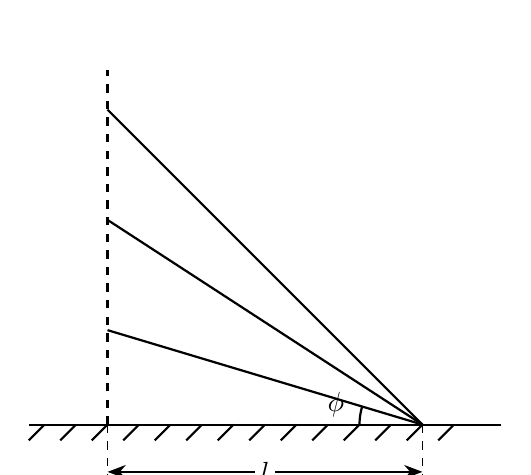
\begin{tikzpicture}[>=Stealth, thick]

    % 定义汇聚点坐标
    \coordinate (A) at (4,0);
    
    % 1. 绘制水平地面线
    \draw (-1,0) -- (5,0);
    
    % 绘制地面的斜线阴影 (表示刚性固定面)
    \foreach \x in {-0.8,-0.4,...,4.8} {
        \draw (\x,0) -- (\x-0.2,-0.2);
    }

    % 2. 绘制竖直虚线
    \draw[dashed] (0,0) -- (0,4.5);

    % 3. 绘制三根连接到地面的斜线
    \draw (0,1.2) -- (A);
    \draw (0,2.6) -- (A);
    \draw (0,4.0) -- (A);

    % 4. 绘制底部的长度标注 l
    % 向下延伸辅助虚线
    \draw[dashed, thin] (0,0) -- (0,-0.8);
    \draw[dashed, thin] (4,0) -- (4,-0.8);
    % 绘制双向箭头及标签
    \draw[<->] (0,-0.6) -- (4,-0.6) node[midway, fill=white, inner sep=2pt] {$l$};

    % 5. 绘制角度 \phi
    % 计算角度: arctan(1.2 / 4) ≈ 16.7°
    % 圆弧中心在 (4,0)，从左侧水平面 (180°) 画到第一根斜线处 (180 - 16.7 = 163.3°)
    \draw (3.2,0) arc[start angle=180, end angle=163.3, radius=0.8];
    \node at (2.9, 0.25) {$\phi$};

\end{tikzpicture}
}\\[4pt]
{\small 图 1-40（题 1-3）}
\end{center}

\newpage

\pdfbookmark[1]{题 1-4}{prob1-4}
\textbf{1-4} 飞机着陆后为尽快停下,采用尾部“降落伞”制动. t=0 刚着陆时的速度大小记为 $v_{0}$ , 坐标取成 $x = 0$ . 假设滑行过程中加速度为 $a_{x} = -\beta v_{x}^{2}$ , 其中 $\beta$ 是正的常量, 试求速度 $v_{x}$ 随位置 $x$ 的变化关系，再求时间 $t$ 的变化关系.

\newpage

\pdfbookmark[1]{题 1-5}{prob1-5}
\textbf{1-5} 在 $x$ 轴上运动的某质点，加速度与位置的关系为 $a_x = -\omega^2 x$ ，其中 $\omega$ 是正的常量. 已知 $t = 0$ 时，质点位于 $x_0 > 0$ 处，速度 $v_0 \neq 0$ ，试求质点位置 $x$ 随时间 $t$ 的变化关系.

\newpage

\pdfbookmark[1]{题 1-6}{prob1-6}
\textbf{1-6} 小球从同一位置以相同的初速率 $v_{0}$ ，在同一竖直平面上朝着不同方向斜抛出去，如果抛射角 $\theta$ 可在 $0 \sim \pi$ 范围内连续变化，试问各轨道最高点连成的曲线是什么类型曲线？

\newpage

\pdfbookmark[1]{题 1-7}{prob1-7}
\textbf{1-7} 一位足球运动员踢出的球具有初速率 25 m/s, 今在球门正前方 50 $m$ 处欲将球踢进球门. 为防止守门员将球挡住, 他选择进球位置在正前方球门水平横梁下方 50 cm 之内区域. 已知横梁高为 2.44 $m$, 试问他应在什么倾角范围将球踢出?

\newpage

\pdfbookmark[1]{题 1-8}{prob1-8}
\textbf{1-8} 一地面雷达观察者正从屏幕上监视由远处投来的一抛射体. 某时刻, 他得到的信息显示: 抛射体达到了最高点且具有水平速度 $v; v$ 的方向线与观察者、抛射体位于同一竖直平面; 抛射体与观察者之间的距离为 $l$ ; 观察者到抛射体连线与水平面的夹角为 $\theta$ .

(1) 预测抛射体落地点与观察者间的水平距离 $d$;

(2) 预测抛射体能否越过观察者的头顶?

\newpage

\pdfbookmark[1]{题 1-9}{prob1-9}
\textbf{1-9} 离地高 $h$ 的大厅吊灯爆炸成碎片，朝各个方向射出，初速度同为 $v_{0}$ . 设吊灯离屋顶和墙较远，碎片不会与之相撞；再设地面铺有毛毯，碎片落地后不会反弹. 试将每一碎片运动斜交地分解成沿其初速 $v_{0}$ 方向的匀速直线运动和静止开始的竖直向下自由落体运动，以此求解地面上碎片分布区域的半径 $R$.

\newpage

\pdfbookmark[1]{题 1-10}{prob1-10}
\textbf{1-10} 质点在 $xy$ 平面上运动, $t = 0$ 时刻, 位于 $x_0 = A, y_0 = 0$ , 速度的两个分量各是 $v_{x0} = 0, v_{y0} = B\omega$ , 任意 $t$ 时刻加速度的两个分量各是 $a_x = -A\omega^2 \cos \omega t, a_y = -B\omega^2 \sin \omega t$ , 其中 $A, B, \omega$ 都是常量, 试求质点运动轨道.

\newpage

\pdfbookmark[1]{题 1-11}{prob1-11}
\textbf{1-11} 查找有关数据,估算下述各量的大小:

(1) 氢原子中电子绕核圆运动的加速度值(绝对值);

(2) 学生匀速骑自行车直线行进时, 车轮边缘点的加速度值;

(3) 以太阳为参考物, 地面上的实验室因地球自转和公转而具有的最大可能的加速度值.

\newpage

\pdfbookmark[1]{题 1-12}{prob1-12}
\textbf{1-12} 半径同为 $R$ 的两个几何球面开始时互相重合, 今使其中一个球面固定, 另一个球面从 t=0 开始匀速平动, 速度大小为 $v_{0}$ .

(1) 试求两球面刚好完全分离的时刻 $t_{e}$ ;

(2) 试求 $0 < t < t_{e}$ 时刻, 两球面交线长度收缩率(单位时间内长度缩短量) $\gamma$ ;

(3) 试求 $0 < t < t_{e}$ 时刻, 两球面交点在第一球面大圆上作圆运动的向心加速度 $a_{\text{心}}$ 和切向加速度 $a_{\text{切}}$ .

\newpage

\pdfbookmark[1]{题 1-13}{prob1-13}
\textbf{1-13} 四质点 $A, B, C, D$ 在同一平面上运动。每一时刻， $A$ 速度总对准 $B$ ，速度大小为常量 $u; B$ 速度总对准 $C$ ，速度大小同为 $u; C$ 速度总对准 $D$ ，速度大小同为 $u; D$ 速度总对准 $A$ ，速度大小同为 $u$ 。某时刻， $A, B, C, D$ 恰好逆时针方向按序位于各边长为 $l$ 的正方形四个顶点上，试求此时 $A$ 的加速度 $a$ 和 $A$ 的运动轨道在此位置的曲率半径 $\rho$ .

\newpage

\pdfbookmark[1]{题 1-14}{prob1-14}
\textbf{1-14} 采用运动学方法, 求解曲线 $y = \mathrm{e}^x$ 的曲率半径随 $x$ 的分布 $\rho(x)$ .

\newpage

\pdfbookmark[1]{题 1-15}{prob1-15}
\textbf{1-15} 在极坐标系中,质点沿着图 1-41 所示的直线以恒定的速度 $v_{0}$ 运动.

(1) 结合图中给出的参量, 写出直线轨道方程 $r-\theta$ ;

(2) 写出质点速度分量 $v_{r}, v_{\theta}$ 与质点角位置 $\theta$ 的关系，再依据加速度分量计算公式，验证 $a_{r}=0, a_{\theta}=0$ .

\begin{center}
\resizebox{0.34\textwidth}{!}{% 1-15 题 图 1-8：极坐标系中质点沿不过极点的直线以恒速 v0 运动
% 直线方程 r cos(θ-θ0)=d，取 θ0=30°、d=2.2（示意），直线 0.866x+0.5y=2.2
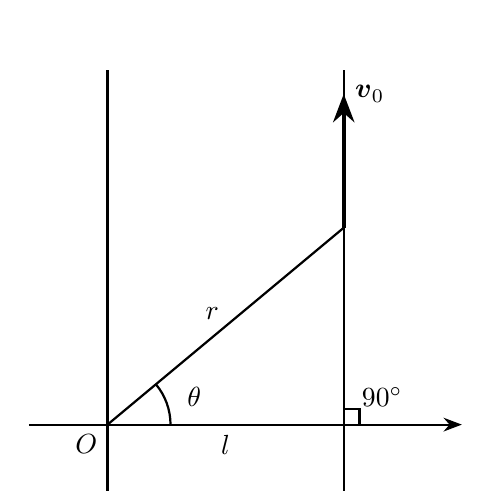
\begin{tikzpicture}[>=Stealth, thick]

    % 定义主要坐标点
    \coordinate (O) at (0,0);       % 原点 O
    \coordinate (A) at (3,0);       % 右侧竖直线与横轴的交点
    \coordinate (B) at (3,2.5);     % 斜线与右侧竖直线的交点

    % 1. 绘制坐标轴和直线
    % 横轴 (带向右的箭头)
    \draw[->] (-1,0) -- (4.5,0);
    
    % 左侧过原点的竖直线
    \draw (0,-1) -- (0,4.5);
    
    % 右侧竖直线
    \draw (3,-1) -- (3,4.5);

    % 2. 绘制斜线 r
    \draw (O) -- (B) node[midway, above left, inner sep=2pt] {$r$};

    % 3. 绘制向上的向量 v_0
    \draw[->, ultra thick] (B) -- (3, 4.2) node[right] {$\boldsymbol{v}_0$};

    % 4. 添加标签 O 和 l
    \node[below left] at (O) {$O$};
    \node[below] at (1.5,0) {$l$};

    % 5. 绘制角度 \theta
    % 半径取 0.8，计算角度大约为 atan(2.5/3) ≈ 39.8°
    \draw (0.8,0) arc[start angle=0, end angle=39.8, radius=0.8];
    \node at (1.1, 0.35) {$\theta$};

    % 6. 绘制直角符号和 90^\circ 标签
    % 在 (3,0) 的右上方画一个边长为 0.2 的直角折线
    \draw (3,0.2) -- (3.2,0.2) -- (3.2,0);
    \node[above right] at (3.1, 0.1) {$90^\circ$};

\end{tikzpicture}
}\\[4pt]
{\small 图 1-41（题 1-15）}
\end{center}

\newpage

\pdfbookmark[1]{题 1-16}{prob1-16}
\textbf{1-16} 以椭圆一个焦点 $F$ 为原点，沿半长轴方向设置极轴，椭圆的极坐标方程是 $r = r_0 / (1 + e\cos \theta)$ . 设所给椭圆的半长轴为 $A$ ，半短轴为 $B$ ，且 $F$ 如图 1-42 所示，位于椭圆中心 $O$ 的右侧.

(1) 确定参量 $r_{0}, e$ 与 $A$, $B$ 的关系；

(2) 若质点以 $\theta=\omega t$ 方式沿椭圆运动，试导出 $v_{\theta}, a_{\theta}$ 与质点角位置 $\theta$ 的关系.

\begin{center}
\resizebox{0.44\textwidth}{!}{% 1-16 题 图 1-9：椭圆，右焦点 F 为极点，极轴沿半长轴方向
% 半长轴 A=3（水平）、半短轴 B=2、焦距 c=sqrt(5)≈2.236（示意比例）
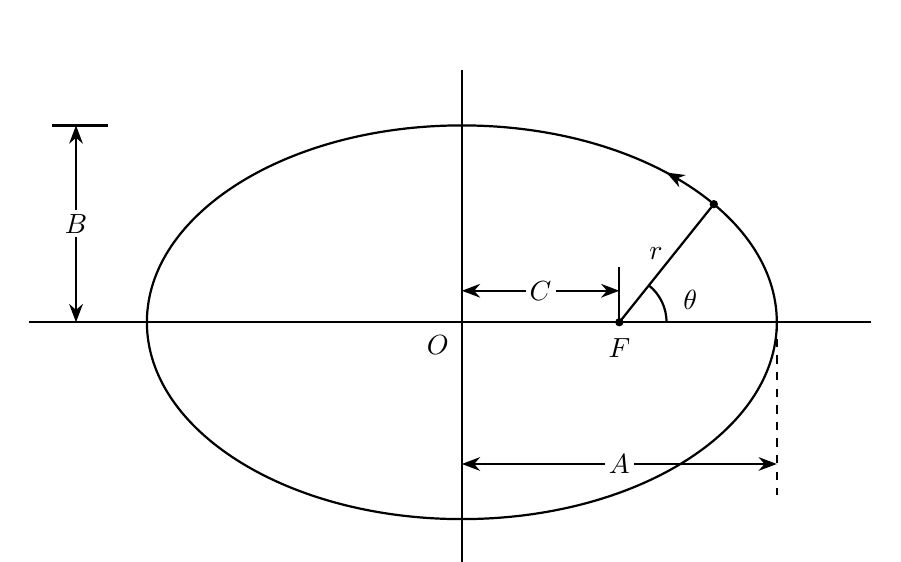
\begin{tikzpicture}[>=Stealth, thick]

    % 定义椭圆的半长轴(a)和半短轴(b)
    \def\a{4}
    \def\b{2.5}
    
    % 定义原点 O 和焦点 F
    \coordinate (O) at (0,0);
    \coordinate (F) at (2,0);
    
    % 定义椭圆上的点 P
    % 选取坐标 (3.2, 1.5)，该点恰好位于 x^2/16 + y^2/6.25 = 1 椭圆上
    \coordinate (P) at (3.2, 1.5);

    % 1. 绘制中心坐标轴 (十字交叉线)
    \draw (-5.5, 0) -- (5.2, 0);
    \draw (0, -3.2) -- (0, 3.2);

    % 2. 绘制带有运动方向箭头的椭圆
    % TikZ 默认逆时针绘制，使用 \arrow{>} 即可实现逆时针箭头指向
    \tikzset{->-/.style={decoration={
      markings,
      mark=at position 0.12 with {\arrow{>}}},postaction={decorate}}}
    \draw[thick, ->-] (O) ellipse ({\a} and {\b});

    % 3. 绘制关键点和位置矢量 r
    \fill (F) circle (1.5pt) node[below=2pt] {$F$};
    \fill (P) circle (1.5pt);
    \node[below left=1pt] at (O) {$O$};
    
    % 绘制 r 连线
    \draw[thick] (F) -- (P) node[midway, above left, inner sep=1pt] {$r$};

    % 4. 绘制角度 \theta
    % P相对F的向量为 (1.2, 1.5)，对应角度 arctan(1.5/1.2) ≈ 51.3°
    \draw (2.6, 0) arc[start angle=0, end angle=51.3, radius=0.6];
    \node at (2.9, 0.28) {$\theta$};

    % 5. 绘制中心到焦点的距离标注 C
    \draw (2,0) -- (2, 0.7); % F 点上方引出的短竖线
    \draw[<->] (0, 0.4) -- (2, 0.4) node[midway, fill=white, inner sep=1.5pt] {$C$};

    % 6. 绘制半长轴标注 A
    \draw[dashed] (\a, 0) -- (\a, -2.2); % 椭圆右边缘向下引出的虚线
    \draw[<->] (0, -1.8) -- (\a, -1.8) node[midway, fill=white, inner sep=1.5pt] {$A$};

    % 7. 绘制半短轴标注 B
    \draw (-4.5, \b) -- (-5.2, \b); % 左上角的短横辅助线
    \draw[<->] (-4.9, 0) -- (-4.9, \b) node[midway, fill=white, inner sep=1.5pt] {$B$};

\end{tikzpicture}
}\\[4pt]
{\small 图 1-42（题 1-16）}
\end{center}

\newpage

\pdfbookmark[1]{题 1-17}{prob1-17}
\textbf{1-17} 平面上有三个动点 $A, B, C, t = 0$ 时刻三者连线构成边长为 $l$ 的等边三角形. 取三角形中心 $O$ 为极坐标系原点, 取 $t = 0$ 时刻 $O$ 到 $A$ 的连线为极轴, 如图 1-43 所示. 若 $A, B, C$ 均在此平面内作匀速率运动, 速率同为 $u$ , 过程中 $A$ 始终朝着 $B$ 运动, $B$ 始终朝着 $C$ 运动, $C$ 始终朝着 $A$ 运动, 试求 $A$ 点运动轨道.

\begin{center}
\resizebox{0.40\textwidth}{!}{% 1-17 题 图 1-10：三个动点构成等边三角形，A 朝 B、B 朝 C、C 朝 A
% 中心 O 为极点，极轴取 O→A；边长 l（示意比例 l=3，外接圆半径 sqrt(3)）
\begin{tikzpicture}[>=Stealth, thick]
    % 定义坐标
    \coordinate (O) at (0,0);
    \coordinate (A) at (3,0);
    \coordinate (B) at (-1.5, 2.6);
    \coordinate (C) at (-1.5, -2.6);

    % 绘制极轴
    \draw[->, thick] (O) -- (4.5,0) node[above] {极轴};
    
    % 绘制虚线三角形
    \draw[dashed] (B) -- (C) node[midway, left] {$l$};
    \draw[dashed] (C) -- (A) node[midway, below right] {$l$};
    \draw[dashed] (A) -- (B) node[midway, above right] {$l$};

    % 绘制实线段 OA
    \draw[thick] (O) -- (A);
    
    % 绘制节点
    \fill (O) circle (1.5pt) node[above left] {$O$};
    \fill (A) circle (1.5pt) node[below right] {$A$};
    \fill (B) circle (1.5pt) node[left] {$B$};
    \fill (C) circle (1.5pt) node[left] {$C$};

    % 绘制速度向量 u (使用粗实线箭头)
    \draw[->, very thick] (B) -- ($(B)!0.4!(C)$) node[left] {$u$};
    \draw[->, very thick] (C) -- ($(C)!0.4!(A)$) node[below right] {$u$};
    \draw[->, very thick] (A) -- ($(A)!0.4!(B)$) node[above left] {$u$};
\end{tikzpicture}
}\\[4pt]
{\small 图 1-43（题 1-17）}
\end{center}

\newpage

\pdfbookmark[1]{题 1-18}{prob1-18}
\textbf{1-18} 极坐标系中方程$r = A (1 - \cos \theta)$,对应一条心脏线, 如图 1-44 所示,试求心底 $P$ 处曲率半径 $\rho$ .

\begin{center}
\resizebox{0.36\textwidth}{!}{% 1-18 题 图 1-12：心脏线 r = A(1-cosθ)，尖点在极点，A 为比例参数（取 A=1.2）
% 心底 P 依题意取尖点正对的圆底（θ=π 处，最左端 (-2A,0)）
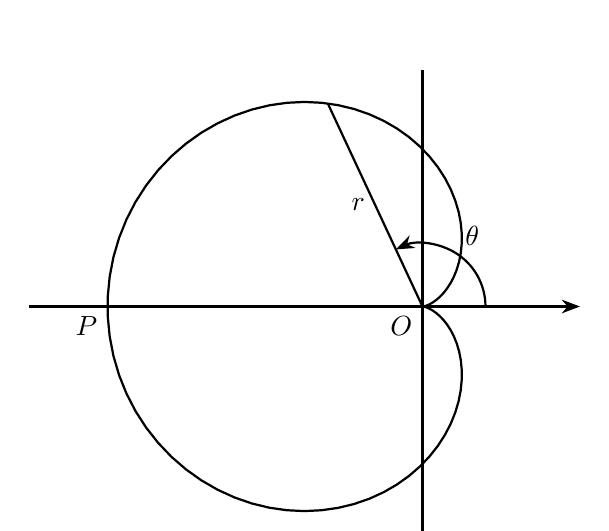
\begin{tikzpicture}[>=Stealth, thick]
    \coordinate (O) at (0,0);
    \coordinate (P) at (-4,0);

    % 绘制坐标轴
    \draw[->] (-5,0) -- (2,0); % 水平轴
    \draw (0,-3) -- (0,3); % 竖直轴

    % 绘制心脏线 r = 2(1 - cos\theta)
    \draw[domain=0:360, samples=100, variable=\t, thick] plot ({\t}: {2*(1-cos(\t))});

    % 绘制 P 和 O 节点
    \node[below left] at (O) {$O$};
    \node[below left] at (P) {$P$};

    % 绘制向径 r 
    \coordinate (R) at (115:{2*(1-cos(115))}); 
    \draw (O) -- (R) node[midway, left] {$r$};
    
    % 绘制 \theta 角度弧
    \draw[->] (0.8,0) arc[start angle=0, end angle=115, radius=0.8];
    \node at (55:1.1) {$\theta$};
\end{tikzpicture}
}\\[4pt]
{\small 图 1-44（题 1-18）}
\end{center}

\newpage

\pdfbookmark[1]{题 1-19}{prob1-19}
\textbf{1-19} 半径 $R$ 的细圆环在半径几乎同为 $R$ 的固定光滑圆柱面外侧面上随意运动, 试求环的自由度.

\newpage

\pdfbookmark[1]{题 1-20}{prob1-20}
\textbf{1-20} 在 $Oxy$ 坐标平面上有一个正三角形和一个正方形, 正三角形和正方形的每条边长相同, 它们的方位如图 1-45 所示. 现在建立一个活动的 $O'x'y'$ 坐标平面, 它的坐标原点开始时位于正三角形的上顶点, 而后 $O'$ 点沿着正三角形的三条边绕行一周. 绕行时, $x'$ 轴始终与 $x$ 轴平行, $y'$ 轴始终与 $y$ 轴平行. 试在图中清楚、准确地画出正四边形相对 $O'x'y'$ 坐标平面运动而形成的区域的边界线.



\begin{center}
\resizebox{0.36\textwidth}{!}{\begin{tikzpicture}[>=Stealth, thick]
    % 主坐标系 O-xy
    \coordinate (O) at (0,0);
    \draw[->] (-3,0) -- (3,0) node[below] {$x$};
    \draw[->] (0,-2.5) -- (0,3) node[left] {$y$};
    \node[below left] at (O) {$O$};

    % 动坐标系 O'-x'y' 参数
    \coordinate (Oprime) at (1.5, 1.5);
    \coordinate (SqCenter) at (-2, -2);
    
    % 绘制连接虚线 (穿过原点 O)
    \draw[dashed] (SqCenter) -- (Oprime);

    % 绘制左下角的正方形 (中心在 SqCenter)
    \draw (-2.3, -1.7) rectangle (-1.7, -2.3);

    % 绘制右上角的三角形 (顶点在 O')
    \draw (Oprime) -- (1.1, 0.7) -- (1.9, 0.7) -- cycle;

    % 绘制 O'-x'y' 坐标轴
    \draw[->] (Oprime) -- (2.8, 1.5) node[right] {$x'$};
    \draw[->] (Oprime) -- (1.5, 2.8) node[right] {$y'$};
    \node[left] at (Oprime) {$O'$};
\end{tikzpicture}}\\[4pt]
{\small 图 1-45（题 1-20）}
\end{center}

\newpage

\pdfbookmark[1]{题 1-21}{prob1-21}
\textbf{1-21} 树上一个苹果离地面高 2.5 $m$, 小孩在距树 1.5 $m$ 处, 从 1.5 $m$ 高度对准苹果抛出一颗小石子的同时, 苹果自由落下. 不计空气阻碍作用, 试问小石子抛出的速度 $v$ 为何值时能击中苹果?

\newpage

\pdfbookmark[1]{题 1-22}{prob1-22}
\textbf{1-22} 风自西向东吹, 风速 $u$ 不变, 一架军用飞机相对于静止大气的飞行速率为恒定的 $v_{0}$ . 设飞机在城市上空沿水平圆轨道巡航飞行, 建立自西向东的 $x$ 轴, 将飞机相对于圆心的径矢与 $x$ 轴夹角记为 $\phi$ , 试求连续的圆轨道飞行条件及轨道速率 $v$ 与方位角 $\phi$ 的关系.

\newpage

\pdfbookmark[1]{题 1-23}{prob1-23}
\textbf{1-23} 刚性的圆环静止在地面上, t=0 时刻开始以恒定的角加速度 $\beta$ 沿直线作纯滚动. 试求任意 t>0 时刻, 环上最高点的加速度大小 $a_{\text{上}}$ 与最低点的加速度大小 $a_{\text{下}}$ 之比值.

\newpage

\pdfbookmark[1]{题 1-24}{prob1-24}
\textbf{1-24} 细杆 $ABC$ 在一竖直平面上靠着一个台阶放着, $A$ 端可沿着水平地面朝台阶运动, 细杆不离开台阶边沿. 当 $ABC$ 杆与水平地面夹角为图 1-46 所示的 $\phi$ 时, 杆的 $B$ 点恰好位于台阶边沿上, 而且 $C$ 端运动速度值恰为 $A$ 端运动速度值的 2 倍, 试求 $BC$ 长与 $AB$ 长的比值 $\alpha$ .


\begin{center}
\resizebox{0.48\textwidth}{!}{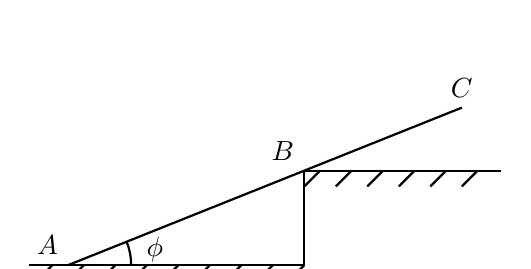
\begin{tikzpicture}[>=Stealth, thick]
    \coordinate (A) at (0,0);
    \coordinate (B) at (3, 1.2);
    \coordinate (C) at (5, 2.0);

    % 绘制地面线 (下层、竖直台阶、上层)
    \draw (-0.5, 0) -- (3, 0); 
    \draw (3, 0) -- (3, 1.2);  
    \draw (3, 1.2) -- (5.5, 1.2); 

    % 绘制下层地面阴影线 (使用 foreach 批量生成)
    \foreach \x in {-0.2, 0.2, 0.6, 1.0, 1.4, 1.8, 2.2, 2.6, 3.0} {
        \draw (\x,0) -- (\x-0.2,-0.2);
    }
    % 绘制上层地面阴影线
    \foreach \x in {3.2, 3.6, 4.0, 4.4, 4.8, 5.2} {
        \draw (\x,1.2) -- (\x-0.2,1.0);
    }

    % 绘制斜杆 AC
    \draw[thick] (A) -- (C);

    % 标注字母
    \node[above left] at (A) {$A$};
    \node[above left] at (B) {$B$};
    \node[above] at (C) {$C$};

    % 绘制角度 \phi (根据几何关系 arctan(1.2/3) ≈ 21.8度)
    \draw (0.8,0) arc[start angle=0, end angle=21.8, radius=0.8];
    \node at (1.1, 0.2) {$\phi$};
\end{tikzpicture}}\\[4pt]
{\small 图 1-46（题 1-24）}
\end{center}

\newpage

\pdfbookmark[1]{题 1-25}{prob1-25}
\textbf{1-25} 4 根长度同为 $l$ 的细杆, 用铰链首尾相接, 组成一个菱形 $ABCD$ , 放在某水平面上, 如图 1-47 所示. 设 $A$ 端固定, $C$ 端沿着 $A$ , $C$ 连线方向运动, 当 $\angle A$ 恰为 $90^{\circ}$ 时, $C$ 端速度为 $v$ , 加速度为 $a$ , 试求此时 $B$ 端的加速度大小 $a_{B}$ .


\begin{center}
\resizebox{0.38\textwidth}{!}{\begin{tikzpicture}[>=Stealth, thick]
    % 定义坐标
    \coordinate (A) at (-3, 0);
    \coordinate (B) at (0, 3);
    \coordinate (C) at (3, 0);
    \coordinate (D) at (0, -3);

    % 绘制虚线对角线
    \draw[dashed] (A) -- (C);
    \draw[dashed] (B) -- (D);

    % 绘制菱形边并标注长度 l
    \draw (A) -- (B) node[midway, above left] {$l$};
    \draw (B) -- (C) node[midway, above right] {$l$};
    \draw (C) -- (D) node[midway, below right] {$l$};
    \draw (D) -- (A) node[midway, below left] {$l$};

    % 绘制节点和字母
    \fill (A) circle (1.5pt) node[left] {$A$};
    \fill (B) circle (1.5pt) node[above] {$B$};
    \fill (C) circle (1.5pt) node[right, yshift=-2mm, xshift=-1mm] {$C$}; 
    \fill (D) circle (1.5pt) node[below] {$D$};

    % 绘制速度和加速度向量 v, a (在 C 的右侧)
    \draw[->, thick] (3.2, 0.4) -- (4.8, 0.4) node[midway, above] {$v$};
    \draw[->, thick] (3.2, -0.4) -- (4.8, -0.4) node[midway, below] {$a$};
\end{tikzpicture}}\\[4pt]
{\small 图 1-47（题 1-25）}
\end{center}


\newpage

\pdfbookmark[1]{题 1-26}{prob1-26}
\textbf{1-26} 在某竖直平面上有一固定的光滑直角三角形细管道 $ABC$ ，小球从顶点 $A$ 沿斜边轨道静止出发自由滑到端点 $C$ 所需时间，恰好等于小球从 $A$ 静止出发自由地经两条直角边轨道滑到 $C$ 所需时间。此处假设竖直轨道 $AB$ 与水平轨道 $BC$ 的交接处为极小的圆弧，可确保小球无碰撞地拐弯，且拐弯时间可略。将 $AB, BC, AC$ 的长分别记作 $L_1, L_2, L_3$ ，试求三者比例关系。

在此直角三角形范围内可构建一系列如图 1-48 所示的光滑折线轨道，每一轨道由若干竖直与水平部分交接而成，交接处有极小圆弧（作用同前），轨道均从 $A$ 到 $C$ ，且不越出该直角三角形边界，试求小球在各条轨道中，自静止出发从 $A$ 滑行到 $C$ 所经时间的上限 $T_{\mathrm{max}}$ 与下限 $T_{\mathrm{min}}$ 之比.

\begin{center}
\resizebox{0.36\textwidth}{!}{% 1-26 题 图1-20：直角三角形管道 + 阶梯形折线轨道
% 直角在 B（AB 竖直, BC 水平），AC 斜边
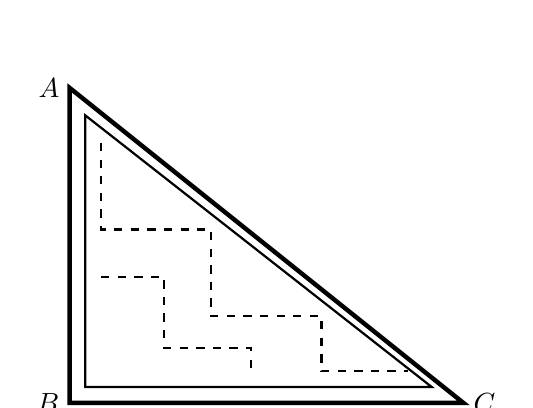
\begin{tikzpicture}[>=Stealth, thick]
    % 外部粗体三角形
    \coordinate (A) at (0,4);
    \coordinate (B) at (0,0);
    \coordinate (C) at (5,0);
    
    \draw[ultra thick] (A) -- (B) -- (C) -- cycle;
    
    % 内部细线三角形框 (模拟中空边框)
    \draw (0.2, 0.2) -- (4.6, 0.2) -- (0.2, 3.65) -- cycle;

    % 标注顶点字母
    \node[left] at (A) {$A$};
    \node[left] at (B) {$B$};
    \node[right] at (C) {$C$};

    % 绘制内部的阶梯形虚线
    % 上层较长的阶梯线
    \draw[dashed] (0.4, 3.3) 
               -- (0.4, 2.2) 
               -- (1.8, 2.2) 
               -- (1.8, 1.1) 
               -- (3.2, 1.1) 
               -- (3.2, 0.4) 
               -- (4.3, 0.4);
               
    % 下层较短的阶梯线
    \draw[dashed] (0.4, 1.6) 
               -- (1.2, 1.6) 
               -- (1.2, 0.7) 
               -- (2.3, 0.7) 
               -- (2.3, 0.4);
\end{tikzpicture}
}\\[4pt]
{\small 图 1-48（题 1-26）}
\end{center}

\newpage

\pdfbookmark[1]{题 1-27}{prob1-27}
\textbf{1-27} 如图 1-49 所示, $A$ 和 $B$ 是两个相同的刚性小球, 开始时 $A$ 和 $B$ 在同一竖直线上, 各自距水平地面的高度分别是 $h_{A}$ 和 $h_{B}$ , 且 $h_{A} > h_{B}$ . 令两球同时从静止自由落下, 而后若两球相碰则彼此交换速度, 若其中一球与地面相碰, 则以原速率反向弹回. 要求 $A$, $B$ 不会与地面一起发生三体碰撞, 试讨论系统形成周期运动的条件.

\begin{center}
\resizebox{0.34\textwidth}{!}{% 1-27 题 图_1_22：两球 A、B 在同一竖直线上自由落下，h_A > h_B
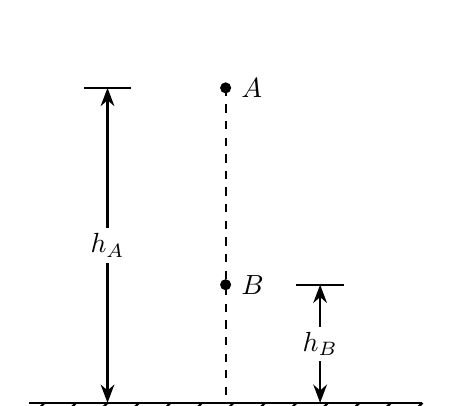
\begin{tikzpicture}[>=Stealth, thick]
    % 绘制地面及其阴影线
    \draw (-2.5, 0) -- (2.5, 0);
    \foreach \x in {-2.3, -1.9, -1.5, -1.1, -0.7, -0.3, 0.1, 0.5, 0.9, 1.3, 1.7, 2.1, 2.5} {
        \draw (\x, 0) -- (\x-0.2, -0.2);
    }

    % 定义点 A 和 B
    \coordinate (A) at (0, 4);
    \coordinate (B) at (0, 1.5);

    % 绘制连接 A 到地面的中心虚线
    \draw[dashed] (A) -- (0, 0);
    
    % 绘制节点 A 和 B 的圆点
    \fill (A) circle (2pt) node[right=2pt] {$A$};
    \fill (B) circle (2pt) node[right=2pt] {$B$};

    % 绘制左侧的 h_A 高度标注
    \draw[<->] (-1.5, 0) -- (-1.5, 4) node[midway, fill=white, inner sep=2pt] {$h_A$};
    % 顶部辅助短横线
    \draw (-1.8, 4) -- (-1.2, 4);

    % 绘制右侧的 h_B 高度标注
    \draw[<->] (1.2, 0) -- (1.2, 1.5) node[midway, fill=white, inner sep=2pt] {$h_B$};
    % 顶部辅助短横线
    \draw (0.9, 1.5) -- (1.5, 1.5);
\end{tikzpicture}
}\\[4pt]
{\small 图 1-49（题 1-27）}
\end{center}

\newpage

\pdfbookmark[1]{题 1-28}{prob1-28}
\textbf{1-28} 长 $L$ 的均匀弹性绳 $AB$ 自由伸直地放在光滑水平桌面上, 绳的 $A$ 端固定. $t = 0$ 时, 一小虫开始从 $A$ 端出发以相对绳的匀速度 $u$ 在绳上朝 $B$ 端爬去, 同时绳的 $B$ 端以匀速度 $v$ 沿绳伸长方向运动, 试求小虫爬到 $B$ 端的时间 $T$ .

\newpage

\pdfbookmark[1]{题 1-29}{prob1-29}
\textbf{1-29} 某人用两手做3个球的抛球、接球、传球游戏. 过程中左手接住空中落下的一个球, 再传递给右手; 右手接过小球, 并将小球斜向上抛出. 假设每只手中至多只留有一个小球, 左手接球点高度与右手抛球点高度相同, 每个小球离开右手后的升高量均达 $H$ , 小球互相不碰撞, 试求系统运动周期 $T$ .

\newpage

\pdfbookmark[1]{题 1-30}{prob1-30}
\textbf{1-30} （1）加速度恒定的运动称为匀加速运动，试证质点的匀加速运动必定是直线运动或者是平面曲线运动,后一种称为匀加速平面曲线运动,简称匀加速曲线运动.

（2）作匀加速曲线运动的质点，在时间 $t_1 = 1\mathrm{s}, t_2 = 2\mathrm{s}, t_3 = 3\mathrm{s}$ 时刻，分别位于空间 $A, B, C$ 点。已知 $\overline{AB} = 8\mathrm{m}, \overline{BC} = 6\mathrm{m}$ ，且 $AB \perp BC$ ，试求质点运动加速度 $\pmb{a}$ 。

\newpage

\pdfbookmark[1]{题 1-31}{prob1-31}
\textbf{1-31} 小物体以初速 $v_{0}$ 、倾角 $\theta$ 斜抛出去，在空气中运动因受阻力而获得与速度 $v$ 反向的附加加速度 $-\gamma v$ ，其中 $\gamma$ 是一个正的常量，试解析给出小物体的运动轨道曲线.

\newpage

\pdfbookmark[1]{题 1-32}{prob1-32}
\textbf{1-32} 设由 $y=y(x)$ 表述的平面曲线，在讨论区域内处处连续，而且 $y' = dy/dx, y'' = d^{2}y/dx^{2}$ 也处处存在并连续，试用运动学方法求解曲率半径分布 $\rho(x)$ .

\newpage

\pdfbookmark[1]{题 1-33}{prob1-33}
\textbf{1-33} 如图 1-50 所示, 岸高 $h$, 人用绳经滑轮拉船靠岸. 若绳与水面夹角为 $\theta$ 时, 人左行速度为 $v_{0}$ , 加速度为 $a_{0}$ (均未必是常量), 试求此时船的左行速度 $v$ 和加速度 $a$.
\begin{center}
\resizebox{0.48\textwidth}{!}{% 1-33 题 图1_25：岸高 h，人用绳经滑轮拉船靠岸，绳与水面夹角 θ
\begin{tikzpicture}[>=Stealth, thick]
    % 地面和悬崖
    \draw (-1, 4) -- (3, 4); % 悬崖顶面
    \draw (3, 4) -- (3, 0);  % 悬崖垂直面
    \draw (3, 0) -- (9, 0);  % 河床底面
    \draw (3, 4) -- (8, 0);  % 斜坡

    % 绘制水面文字
    \node[below] at (6, 0) {河水};

    % 左侧站立的小人
    \draw (0.8, 4.5) circle (0.15); % 头
    \draw (0.8, 4.35) -- (0.8, 4.15); % 躯干
    \draw (0.8, 4.15) -- (0.7, 4.0); % 左腿
    \draw (0.8, 4.15) -- (0.9, 4.0); % 右腿
    \draw (0.6, 4.25) -- (1.0, 4.25); % 胳膊

    % 右侧边缘处的小人/物体 (蹲伏状)
    \draw (2.8, 4.25) circle (0.12);
    \draw (2.8, 4.13) -- (2.7, 4.0);
    \draw (2.8, 4.13) -- (2.9, 4.0);
    \draw (2.6, 4.15) -- (3.0, 4.15);

    % 速度和加速度向量
    \draw[->, thick] (1.2, 4.8) -- (0.2, 4.8) node[midway, above] {$v_0, a_0$};

    % 高度 h 标注
    \draw (2.3, 4) -- (2.9, 4); % 上辅助线
    \draw (2.3, 0) -- (2.9, 0); % 下辅助线
    \draw[<->] (2.6, 0) -- (2.6, 4) node[midway, fill=white, inner sep=2pt] {$h$};

    % 角度 \theta
    \draw (7.2, 0) arc[start angle=180, end angle=141.3, radius=0.8]; % arctan(4/5) ≈ 38.7°, 180-38.7 = 141.3°
    \node at (7.5, 0.3) {$\theta$};
\end{tikzpicture}
}\\[4pt]
{\small 图 1-50（题 1-33）}
\end{center}

\newpage

\pdfbookmark[1]{题 1-34}{prob1-34}
\textbf{1-34} 极坐标系中的对数螺线可表述为 $r=r_{0}e^{\alpha\theta}$ ，试用运动学方法导出曲率半径分布 $\rho(r)$ .

\newpage

\pdfbookmark[1]{题 1-35}{prob1-35}
\textbf{1-35} 空间光滑连续曲线上取三个点, 可确定一个平面, 这三个点无限靠近时确定的极限平面记为 $\sigma$ , 曲线上由这三个点的两个端位点界定的无穷小曲线段必定都在 $\sigma$ 平面内, 并可逼近处理成无穷小圆弧段, 圆半径便是这一空间曲线在此位置处的曲率半径.

等距螺旋线的曲率半径必定处处相同,试用运动学方法,求解旋转圆半径和螺距分别为 $R$ 和 $H$ 的等距螺旋线的曲率半径 $\rho$ .

\newpage

\pdfbookmark[1]{题 1-36}{prob1-36}
\textbf{1-36} 如图 1-51 所示, 轰炸机 $A$ 以速度 $v_{1}$ 作水平匀速飞行, 飞行高度为 $H$.

(1) 为使自由释放的炸弹击中地面目标 $B$，应在距 $B$ 多远的水平距离 $L$ 处投弹？（2）在地面上与 $B$ 相距 $D$ 处有一高射炮 $C$，在 $A$ 释放炸弹同时发射炮弹，为使炮弹能击中飞行中的炸弹，试问炮弹初速 $v_{2}$ 至少为多大？若 $v_{2}$ 取最小值，炮弹发射角 $\gamma$ 为多大？
\begin{center}
\resizebox{0.40\textwidth}{!}{% 1-36 题 图1_30：轰炸机 A 水平飞行高度 H，炸弹击中 B；高射炮 C 距 B 为 D
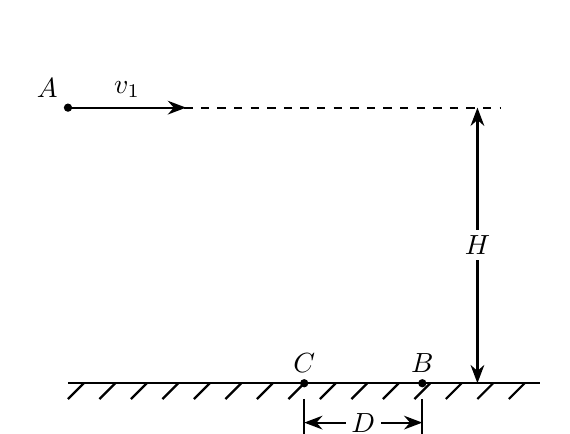
\begin{tikzpicture}[>=Stealth, thick]
    % 地面及阴影
    \draw (0, 0) -- (6, 0);
    \foreach \x in {0.2, 0.6, 1.0, 1.4, 1.8, 2.2, 2.6, 3.0, 3.4, 3.8, 4.2, 4.6, 5.0, 5.4, 5.8} {
        \draw (\x, 0) -- (\x-0.2, -0.2);
    }

    % 点 A 和平抛虚线
    \coordinate (A) at (0, 3.5);
    \fill (A) circle (1.5pt) node[above left] {$A$};
    \draw[dashed, thick] (A) -- (5.5, 3.5);

    % 速度向量 v1
    \draw[->, thick] (A) -- (1.5, 3.5) node[midway, above] {$v_1$};

    % 高度 H 标注
    \draw[<->] (5.2, 0) -- (5.2, 3.5) node[midway, fill=white, inner sep=2pt] {$H$};

    % 地面上的点 C 和 B
    \coordinate (C) at (3, 0);
    \coordinate (B) at (4.5, 0);
    \fill (C) circle (1.5pt) node[above] {$C$};
    \fill (B) circle (1.5pt) node[above] {$B$};

    % 距离 D 标注
    \draw (3, -0.2) -- (3, -0.8);
    \draw (4.5, -0.2) -- (4.5, -0.8);
    \draw[<->] (3, -0.5) -- (4.5, -0.5) node[midway, fill=white, inner sep=2pt] {$D$};
\end{tikzpicture}
}\\[4pt]
{\small 图 1-51（题 1-36）}
\end{center}

\newpage

\pdfbookmark[1]{题 1-37}{prob1-37}
\textbf{1-37} 惠更斯等时摆.

半径 $R$ 的轮子在水平直线 MN 上方纯滚动, 轮子边缘上任意点 $P$ 的运动轨迹不妨称为上滚轮线. 如图 1-52 所示, 将上滚轮线绕 MN 向下翻转 $180^{\circ}$ , 成为下滚轮线. 下滚轮线也可看成 $R$ 轮子在下方沿直线 MN 纯滚动时轮子边缘点 $P$ 的运动轨迹.

沿下滚轮线设置光滑轨道, 小球在轨道内侧除最低点外任意一处从静止自由滑下, 可形成周期性的往返运动(摆动), 惠更斯已证得摆动周期 $T$ 与小球初始位置无关, 后人将此种摆称为惠更斯等时摆. 试在认知等时性前提下, 求出以 $R$ 为参量的 $T$ 算式.

\begin{center}
\resizebox{0.55\textwidth}{!}{% 1-37 题 图1-52：惠更斯等时摆——上滚轮线与下滚轮线
% 轮半径 R=1（TikZ 单位）。上滚轮线：摆线 x=R(t-sin t), y=R(1-cos t), t∈[0,2π]，尖点落在 MN 上；
% 下滚轮线：上滚轮线关于 MN 翻转 180°（图中虚线）。
\begin{tikzpicture}[>=Stealth, thick, scale=1.0]
    % 水平直线 MN
    \draw (-0.6, 0) -- (7.2, 0);
    \node[left] at (-0.6, 0) {$M$};
    \node[right] at (7.2, 0) {$N$};

    % 上滚轮线（实线）
    \draw[thick, domain=0:360, samples=160, variable=\t]
        plot ({(\t*pi/180) - sin(\t)}, {1 - cos(\t)});
    % 下滚轮线（关于 MN 翻转，虚线）
    \draw[thick, dashed, domain=0:360, samples=160, variable=\t]
        plot ({(\t*pi/180) - sin(\t)}, {-(1 - cos(\t))});

    % 生成圆（轮子位于拱顶处）
    \draw[thin, dashed] (3.1416, 1) circle (1);
    \fill (3.1416, 1) circle (1pt) node[right=1pt] {$O$};
    \fill (3.1416, 2) circle (1.5pt) node[above] {$P$};
    \draw[->, thin] (3.1416, 1) -- (3.1416, 2) node[midway, right] {$R$};

    % 曲线名称
    \node[right] at (6.5, 1.7) {\small 上滚轮线};
    \node[right] at (6.5, -1.7) {\small 下滚轮线};
\end{tikzpicture}
}\\[4pt]
{\small 图 1-52（题 1-37）}
\end{center}

% FIGSCALE 0.8 / BOOKMARKS
\chapter{牛顿定律 动量定理}

\pdfbookmark[1]{题 2-1}{prob2-1}
\textbf{2-1} 如图 2-43 所示, 一轻绳跨过光滑的定滑轮, 绳的两端等高处分别有一个胖猴和瘦猴, 两猴身高相同. 胖猴使劲沿着绳向上爬, 瘦猴懒洋洋地挂在绳上, 试问吊在滑轮下边的香蕉将归谁所有?

\begin{center}
\resizebox{0.26\textwidth}{!}{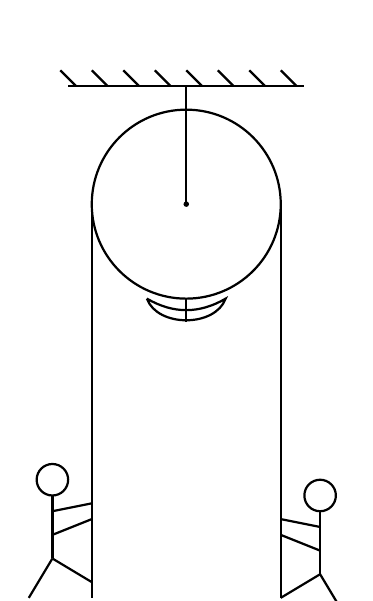
\begin{tikzpicture}[>=Stealth, thick]
    % 天花板
    \draw (-1.5, 4) -- (1.5, 4);
    \foreach \x in {-1.4, -1.0, -0.6, -0.2, 0.2, 0.6, 1.0, 1.4} {
        \draw (\x, 4) -- (\x-0.2, 4.2);
    }

    % 悬挂线和滑轮
    \draw (0, 4) -- (0, 2.5);
    \draw (0, 2.5) circle (1.2);
    \fill (0, 2.5) circle (1pt); % 中心点

    % 底部月牙形挂钩/结构
    \draw[thick] (-0.5, 1.3) to[out=-70, in=250] (0.5, 1.3) to[out=210, in=-30] (-0.5, 1.3);
    \draw (0, 1.3) -- (0, 1.0); % 连接杆

    % 两侧的绳子
    \draw (-1.2, 2.5) -- (-1.2, -2.5);
    \draw (1.2, 2.5) -- (1.2, -2.5);

    % 左侧攀爬的小人
    \draw (-1.7, -1.0) circle (0.2); % 头
    \draw (-1.7, -1.2) -- (-1.7, -2.0); % 躯干
    \draw (-1.7, -1.4) -- (-1.2, -1.3); % 胳膊 1
    \draw (-1.7, -1.7) -- (-1.2, -1.5); % 胳膊 2
    \draw (-1.7, -2.0) -- (-2.0, -2.5); % 腿 1 (向外)
    \draw (-1.7, -2.0) -- (-1.2, -2.3); % 腿 2 (踩绳)

    % 右侧攀爬的小人
    \draw (1.7, -1.2) circle (0.2); % 头
    \draw (1.7, -1.4) -- (1.7, -2.2); % 躯干
    \draw (1.7, -1.6) -- (1.2, -1.5); % 胳膊 1
    \draw (1.7, -1.9) -- (1.2, -1.7); % 胳膊 2
    \draw (1.7, -2.2) -- (2.0, -2.7); % 腿 1 (向外)
    \draw (1.7, -2.2) -- (1.2, -2.5); % 腿 2 (踩绳)
\end{tikzpicture}
}\\[4pt]
{\small 图 2-43（题 2-1）}
\end{center}

\newpage

\pdfbookmark[1]{题 2-2}{prob2-2}
\textbf{2-2} 天花板下悬挂轻质光滑小圆环 $P, P$ 可绕着过悬挂点的竖直轴无摩擦地旋转，长为 $L$ 的轻绳穿过 $P$ ，两端分别连接质量 $m_{1}$ 和 $m_{2}$ 的小球. 设两球同时作图 2-44 所示的圆锥摆运动，且在任意时刻两球和绳均在同一个竖直平面内，试求两小球各自到 $P$ 点的距离 $l_{1}$ 和 $l_{2}$ .

\begin{center}
\resizebox{0.44\textwidth}{!}{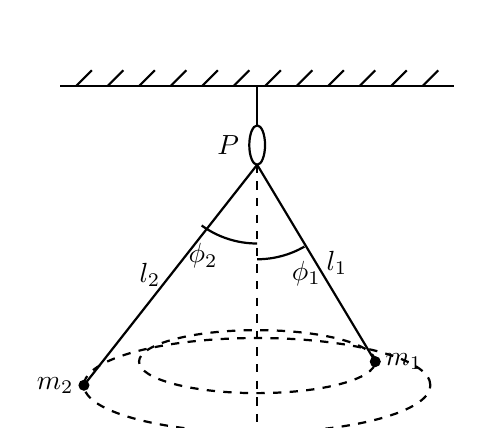
\begin{tikzpicture}[>=Stealth, thick]
    % Ceiling
    \draw (-2.5, 4) -- (2.5, 4);
    \foreach \x in {-2.3, -1.9, ..., 2.3} \draw (\x, 4) -- (\x+0.2, 4.2);
    
    % Hanger & Point P
    \draw (0, 4) -- (0, 3.5);
    \draw (0, 3.25) ellipse (0.1 and 0.25);
    \node[left] at (-0.1, 3.25) {$P$};
    \coordinate (P) at (0, 3);
    
    % Vertical dashed line
    \draw[dashed] (P) -- (0, -0.5);
    
    % Masses
    \coordinate (M1) at (1.5, 0.5);
    \coordinate (M2) at (-2.2, 0.2);
    
    \draw (P) -- (M1) node[midway, right] {$l_1$};
    \draw (P) -- (M2) node[midway, left] {$l_2$};
    \fill (M1) circle (2pt) node[right] {$m_1$};
    \fill (M2) circle (2pt) node[left] {$m_2$};
    
    % Ellipses
    \draw[dashed] (0, 0.5) ellipse (1.5 and 0.4);
    \draw[dashed] (0, 0.2) ellipse (2.2 and 0.6);
    
    % Angles
    % phi1 and phi2 arcs (fixed arc syntax)
    \draw (0,1.8) arc[start angle=270, end angle=300, radius=1.2] node[pos=0.5, below right, yshift=2pt] {$\phi_1$};
    \draw (0,2.0) arc[start angle=270, end angle=234, radius=1.2] node[pos=0.5, below left, yshift=2pt] {$\phi_2$};
\end{tikzpicture}}\\[4pt]
{\small 图 2-44（题 2-2）}
\end{center}

\newpage

\pdfbookmark[1]{题 2-3}{prob2-3}
\textbf{2-3} 质量 $m$, 长 $l$ 的匀质细杆 OA, 在光滑的水平面上绕其固定端 $O$ 旋转, 旋转角速度为 $\omega$ 常量. 以 $O$ 端为原点, 在杆上建立沿 OA 方向的 $x$ 轴, 试求细杆中张力 $T$ 随 $x$ 的分布函数.

\newpage

\pdfbookmark[1]{题 2-4}{prob2-4}
\textbf{2-4} 估算月球中心到地球中心的距离 $r$.

\newpage

\pdfbookmark[1]{题 2-5}{prob2-5}
\textbf{2-5} $A$, $B$ 两本书各 300 张, 每张质量 3 $g$, 纸间摩擦因数同为 $\mu=0.3$ . 将 $A$, $B$ 两书逐张交叠放在光滑水平桌面上, 试问为将两书水平拉开至少要用多大的力?

\newpage

\pdfbookmark[1]{题 2-6}{prob2-6}
\textbf{2-6} 如图 2-45 所示,传送带水平段长度为 $l$,传动速度为 $v_{0}$ ,小物块无水平初速地放在传送带的左端,经时间 $t$ 到达右端.已知小物块与传送带之间的摩擦因数处处相同,试求小物块到达右端时的速度 $v$ 及摩擦因数 $\mu$ .

\begin{center}
\resizebox{0.50\textwidth}{!}{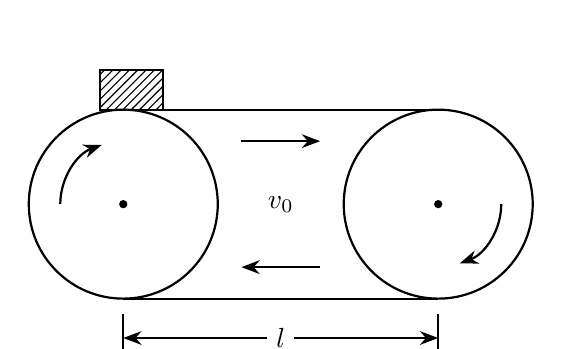
\begin{tikzpicture}[>=Stealth, thick]
    \coordinate (O1) at (0, 0);
    \coordinate (O2) at (4, 0);
    \def\R{1.2}
    
    % Pulleys
    \draw (O1) circle (\R);
    \draw (O2) circle (\R);
    \fill (O1) circle (1.5pt);
    \fill (O2) circle (1.5pt);
    
    % Belt
    \draw (0, \R) -- (4, \R);
    \draw (0, -\R) -- (4, -\R);
    
    % Rotation arrows
    \draw[->] (-0.8, 0) arc[start angle=180, end angle=110, radius=0.8];
    \draw[->] (4.8, 0) arc[start angle=0, end angle=-70, radius=0.8];
    
    % Belt movement arrows
    \draw[->] (1.5, 0.8) -- (2.5, 0.8);
    \draw[->] (2.5, -0.8) -- (1.5, -0.8);
    \node at (2, 0) {$v_0$};
    
    % Block
    \draw[pattern=north east lines] (-0.3, \R) rectangle (0.5, \R+0.5);
    \draw[thick] (-0.3, \R) rectangle (0.5, \R+0.5);
    
    % Dimensions
    \draw (0, -\R-0.2) -- (0, -\R-0.8);
    \draw (4, -\R-0.2) -- (4, -\R-0.8);
    \draw[<->] (0, -\R-0.5) -- (4, -\R-0.5) node[midway, fill=white] {$l$};
\end{tikzpicture}
}\\[4pt]
{\small 图 2-45（题 2-6）}
\end{center}

\newpage

\pdfbookmark[1]{题 2-7}{prob2-7}
\textbf{2-7} 底圆半顶角为 $\theta$ 的圆锥形筒水平倒置，绕其竖直中央轴以恒定的角速度 $\omega$ 旋转，在筒内侧面距筒顶 $l$ 处放一小物块，如图 2-46 所示.设物块与筒间摩擦因数为 $\mu$ ，试问 $l$ 取何值时，小物块能相对筒静止？

\begin{center}
\resizebox{0.30\textwidth}{!}{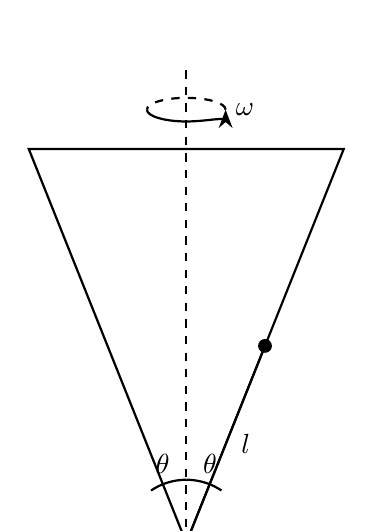
\begin{tikzpicture}[>=Stealth, thick]
    \coordinate (V) at (0, -3); % Vertex
    \coordinate (TL) at (-2, 2);
    \coordinate (TR) at (2, 2);
    
    \draw (TL) -- (TR) -- (V) -- cycle;
    \draw[dashed] (0, 3) -- (V);
    
    % Omega arrow
    \draw[->] (-0.5, 2.5) arc[start angle=180, end angle=360, x radius=0.5, y radius=0.15] node[right] {$\omega$};
    \draw[dashed] (0.5, 2.5) arc[start angle=0, end angle=180, x radius=0.5, y radius=0.15];
    
    % Angles
    \draw (0, -2.2) arc[start angle=90, end angle=124, radius=0.8];
    \node at (-0.3, -2.0) {$\theta$};
    \draw (0, -2.2) arc[start angle=90, end angle=56, radius=0.8];
    \node at (0.3, -2.0) {$\theta$};
    
    % Mass
    \coordinate (M) at (1, -0.5);
    \fill (M) circle (2.5pt);
    \draw (V) -- (M) node[midway, right, xshift=2pt] {$l$};
\end{tikzpicture}}\\[4pt]
{\small 图 2-46（题 2-7）}
\end{center}

\newpage

\pdfbookmark[1]{题 2-8}{prob2-8}
\textbf{2-8} 将小物块放在水平转盘距中心 $r_{1}=0.10\ m$ 处，转盘以 $\beta=20\ rad/s^{2}$ 的角加速度绕着过中心的竖直轴旋转，当角速度达到 $\omega=7.0\ rad/s$ 时，小物块开始滑动。如果小物块开始时放在距盘心 $r_{2}=0.15\ m$ 处，摩擦因数不变，盘的旋转情况同前，问达到多大角速度 $\omega_{2}$ 时，小物块开始滑动？

\newpage

\pdfbookmark[1]{题 2-9}{prob2-9}
\textbf{2-9} 高台跳水运动员入水后, 当向下的速度降到约 $2 \mathrm{~m} / \mathrm{s}$ 时翻身, 并以双脚蹬池底向上浮出水面为宜. 运动员在水中所受阻力可近似表述为 $\frac{1}{2} C \rho S v^{2}$ , 其中 $C = 0.5$ 是阻力系数, $\rho$ 是人体密度, $S$ 是人体垂直于运动方向的截面积, $v$ 是运动速率, 试为女子 $10 \mathrm{~m}$ 高台跳水设计游泳池的深度.

\newpage

\pdfbookmark[1]{题 2-10}{prob2-10}
\textbf{2-10} 光滑的水平面上放一个大三角形木块, 在木块的光滑斜面上放一个小长方木块. 将两者从静止自由释放, 试利用平移惯性力建立小长方木块相对大三角形木块的动力学方程, 以协助判定小长方木块到达地面前是否会离开大木块.

\newpage

\pdfbookmark[1]{题 2-11}{prob2-11}
\textbf{2-11} 车厢内的滑轮装置如图 2-47 所示, 滑轮固定不转动, 只是为轻绳提供光滑的接触. 物块 $A$ 与水平桌面间摩擦因数 $\mu=0.25$ , $A$ 的质量 $m_{A}=20\ kg$ , 物块 $B$ 的质量 $m_{B}=30\ kg$ . 今使车厢沿图示水平朝左方向匀加速运动, 加速度 $a_{0}=2\ m/s^{2}$ , 稳定后绳将倾斜不晃, 试求绳中张力 $T$.

\begin{center}
\resizebox{0.50\textwidth}{!}{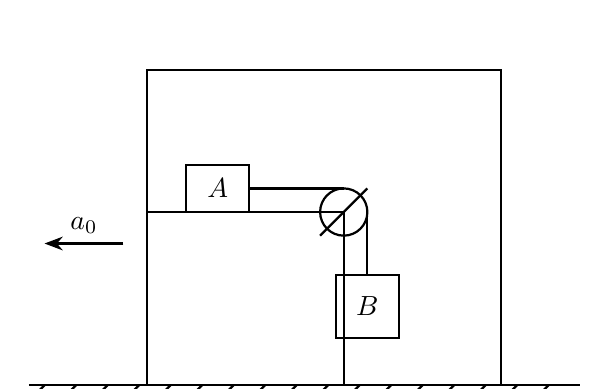
\begin{tikzpicture}[>=Stealth, thick]
    % 地面及阴影线
    \draw (-1.5, 0) -- (5.5, 0);
    \foreach \x in {-1.3, -0.9, ..., 5.3} {
        \draw (\x, 0) -- (\x-0.2, -0.2);
    }
    
    % 主机架外框
    \draw (0, 0) rectangle (4.5, 4);
    
    % 机架内侧的阶梯状转折
    \draw (0, 2.2) -- (2.5, 2.2) -- (2.5, 0);
    
    % 定滑轮及轴心标志
    \coordinate (C) at (2.5, 2.2);
    \draw (C) circle (0.3);
    \draw (2.2, 1.9) -- (2.8, 2.5);
    
    % 物块 A (放置在水平架上)
    \draw[thick] (0.5, 2.2) rectangle (1.3, 2.8) node[midway] {$A$};
    
    % 物块 B (悬挂在竖直侧)
    \draw[thick] (2.4, 0.6) rectangle (3.2, 1.4) node[midway] {$B$};
    
    % 连接滑轮的细线
    \draw (1.3, 2.5) -- (2.5, 2.5); % 水平段
    \draw (2.8, 2.2) -- (2.8, 1.4); % 竖直段
    
    % 整体的加速度 a_0
    \draw[->, thick] (-0.3, 1.8) -- (-1.3, 1.8) node[midway, above] {$a_0$};
\end{tikzpicture}}\\[4pt]
{\small 图 2-47（题 2-11）}
\end{center}

\newpage

\pdfbookmark[1]{题 2-12}{prob2-12}
\textbf{2-12} 游乐场中的转笼是一个半径 3 $m$ 的直立圆筒, 可绕中央竖直轴旋转, 游客可背靠筒壁站立在水平踏板上, 筒壁上有粗糙的网纹以增大游客与筒壁之间的摩擦因数 $\mu$ . 当转速达到每分钟 30 转时, 游客脚下踏板脱落, 从转笼参考系考虑, 为使游客不会掉下落地, 试问 $\mu$ 至少为多大?

\newpage

\pdfbookmark[1]{题 2-13}{prob2-13}
\textbf{2-13} 不计空气阻力, 近似计算小球从赤道上空 100 $m$ 高处自由下落时, 因受科里奥利力影响产生的落地偏东值. (数学处理时,可利用复合函数微商链锁法则： $\frac{\mathrm{d}y}{\mathrm{d}x} = \frac{\mathrm{d}y}{\mathrm{d}u} \frac{\mathrm{d}u}{\mathrm{d}x}$)

\newpage

\pdfbookmark[1]{题 2-14}{prob2-14}
\textbf{2-14} 以角速度 $\omega$ 绕着过中心竖直轴匀速旋转的水平大圆盘上有一弦心距为 $d$ 的足够长直弦槽，槽内有一个质量 $m$ 的小物块从槽的中央 $O$ 处以初始相对速率 $v_{0}$ 沿槽运动。已知小物块与槽的侧壁光滑接触，与槽底间的摩擦因数为 $\mu$ 。试问 $\mu$ 为何值，小物块最终能停住？再设所给 $\mu$ 值能使小物块停住，试导出小物块滑动时槽的侧壁所受正压力大小 $N$ 与物块经过的路程 $x$ 之间的关系，并计算小物块通过的总路程 $s$ 。

\newpage

\pdfbookmark[1]{题 2-15}{prob2-15}
\textbf{2-15} 半长轴为 $a$、半短轴为 $b$ 的椭圆，长轴端点处的曲率半径 $\rho=b^{2}/a$ .质量 $m$ 的人造卫星绕地球作椭圆运动, 近地点离地面的高度为 2R, 远地点离地面的高度为 3R, 其中 $R$ 是地球半径. 已知地球表面处重力加速度为 $g$, 试求人造卫星从远地点到近地点运行过程中, 地球万有引力给它的总冲量大小 $I$.

\newpage

\pdfbookmark[1]{题 2-16}{prob2-16}
\textbf{2-16} 光滑水平地面上有一个倾角 $\phi$ 、高 $H$ 、质量 $M$ 的劈形木块, 它的顶部有一质量 $m$ 的小物块, 两者间有摩擦. 开始时系统静止, 如图 2-48 所示, 而后小物块能够沿斜面下滑到底部, 试求过程中劈形木块在地面上通过的路程 $s$.

\begin{center}
\resizebox{0.47\textwidth}{!}{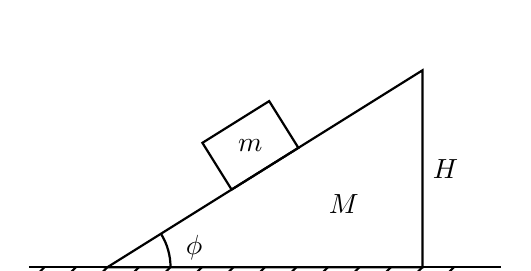
\begin{tikzpicture}[>=Stealth, thick]
    % 地面及阴影线
    \draw (-1, 0) -- (5, 0);
    \foreach \x in {-0.8, -0.4, ..., 4.8} {
        \draw (\x, 0) -- (\x-0.2, -0.2);
    }
    
    % 斜面及其质量标注 M
    \coordinate (A) at (0, 0);
    \coordinate (B) at (4, 0);
    \coordinate (C) at (4, 2.5);
    \draw (A) -- (B) -- (C) -- cycle;
    \node at (3, 0.8) {$M$};
    
    % 高度 H
    \node[right] at (4, 1.25) {$H$};
    
    % 坡角 \phi
    \draw (0.8, 0) arc (0:32:0.8);
    \node at (1.1, 0.25) {$\phi$};
    
    % 斜面上的物块 m
    \begin{scope}[shift={(2, 1.25)}, rotate=32]
        \draw[thick] (-0.5, 0) rectangle (0.5, 0.7) node[midway] {$m$};
    \end{scope}
\end{tikzpicture}}\\[4pt]
{\small 图 2-48（题 2-16）}
\end{center}

\newpage

\pdfbookmark[1]{题 2-17}{prob2-17}
\textbf{2-17} 炮车以仰角 $\alpha$ 发射一炮弹, 两者质量分别为 $M$ 和 $m$. 已知炮弹出口时相对地面速度大小为 $v$, 略去炮车与水平地面间的摩擦, 试求炮车反冲速度 $v_{0}$ .

\newpage

\pdfbookmark[1]{题 2-18}{prob2-18}
\textbf{2-18} 平直轨道上停着一节质量 $M = 20m$ 的车厢, 车厢与铁轨间摩擦可略. 有 $N$ 名学生列队前行, 教员在最后, 每名学生的质量同为 $m$ . 当他们发现前面车厢时, 都以相同速度 $v_{0}$ 跑步, 每名学生在接近车厢时又以 $2v_{0}$ 速度跑着上车坐下, 教员却因跑步速度没有改变而恰好未能上车, 试求 $N$ .

\newpage

\pdfbookmark[1]{题 2-19}{prob2-19}
\textbf{2-19} 从喷泉中喷出的水柱, 把一个质量 $m$ 的圆筒倒顶在空中, 如图 2-49 所示. 水以恒定的速率 $v_{0}$ 从面积为 $S$ 的小孔喷出, 射向空中, 在冲击桶底后, 一半水附在桶底, 随即顺内壁流下, 其速度可略, 另一半水则以原速竖直溅下. 将水的密度记为 $\rho$ , 试求桶停留的高度 $H$.

\begin{center}
\resizebox{0.36\textwidth}{!}{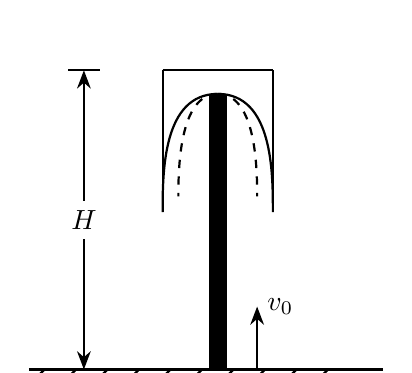
\begin{tikzpicture}[>=Stealth, thick]
    % Ground
    \draw (-1.5, 0) -- (3, 0);
    \foreach \x in {-1.3, -0.9, ..., 2.7} \draw (\x, 0) -- (\x-0.2, -0.2);
    
    % Fountain jet
    \draw (0.8, 0) -- (0.8, 3.5); % left edge of main jet
    \draw (1.0, 0) -- (1.0, 3.5); % right edge of main jet
    \fill (0.8, 0) rectangle (1.0, 3.5); % Solid jet core
    
    % Water arcs
    % Outer arcs
    \draw (0.9, 3.5) .. controls (0.2, 3.5) and (0.2, 2.5) .. (0.2, 2.0);
    \draw (0.9, 3.5) .. controls (1.6, 3.5) and (1.6, 2.5) .. (1.6, 2.0);
    % Inner dashed arcs
    \draw[dashed] (0.9, 3.5) .. controls (0.4, 3.5) and (0.4, 2.5) .. (0.4, 2.2);
    \draw[dashed] (0.9, 3.5) .. controls (1.4, 3.5) and (1.4, 2.5) .. (1.4, 2.2);
    
    % Top flat line bounding the fountain
    \draw (0.2, 3.8) -- (1.6, 3.8);
    \draw (0.2, 3.8) -- (0.2, 2.0);
    \draw (1.6, 3.8) -- (1.6, 2.0);
    
    % Height H
    \draw[<->] (-0.8, 0) -- (-0.8, 3.8) node[midway, fill=white] {$H$};
    % Helper arrows at top and bottom for H
    \draw (-1.0, 3.8) -- (-0.6, 3.8);
    
    % v0 arrow
    \draw[->] (1.4, 0) -- (1.4, 0.8) node[right] {$v_0$};
\end{tikzpicture}}\\[4pt]
{\small 图 2-49（题 2-19）}
\end{center}

\newpage

\pdfbookmark[1]{题 2-20}{prob2-20}
\textbf{2-20} 质量 $m_{0}$ 、初速 $v_{0}$ 的无动力飞行器在太空尘埃中运动，运动过程中飞行器会吸附尘埃，吸附质量与路程成正比，比例系数为常量 $\alpha$ .

(1) 确定飞行器停止前通过的总路程；

(2) 确定飞行器运动速度与时间的关系.

\newpage

\pdfbookmark[1]{题 2-21}{prob2-21}
\textbf{2-21} 长 $l$ 、质量线密度为 $\lambda$ 的匀质软绳，开始时两端 $A$ 和 $B$ 一起悬挂在固定点上。使 $B$ 端脱离悬挂点自由下落，当如图 2-50 所示， $B$ 端下落高度 $x < l$ 时，试求悬挂点所受拉力 $T$ 的大小。

\begin{center}
\resizebox{0.34\textwidth}{!}{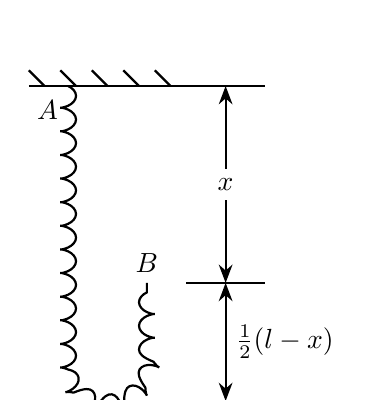
\begin{tikzpicture}[>=Stealth, thick]
    % Ceiling
    \draw (-0.5, 4) -- (1.5, 4);
    \foreach \x in {-0.3, 0.1, 0.5, 0.9, 1.3} \draw (\x, 4) -- (\x-0.2, 4.2);
    
    \node[left] at (0, 3.7) {$A$};
    \node[above] at (1, 1.5) {$B$};
    
    % Chain drawing using small ellipses
    \def\chainy{
        \foreach \i in {0,...,25} {
            \draw[rotate around={90:(0, 3.8 - \i*0.15)}] (0, 3.8 - \i*0.15) ellipse (0.05 and 0.1);
        }
        % Bottom loop
        \foreach \i in {0,...,8} {
            \draw[rotate around={180-\i*22.5:(0.5, 0.05)}] ({0.5 + 0.5*cos(180-\i*22.5)}, {0.05 + 0.5*sin(180-\i*22.5)}) ellipse (0.05 and 0.1);
        }
        % Right side going up to B
        \foreach \i in {0,...,9} {
            \draw[rotate around={90:(1, 0.05 + \i*0.15)}] (1, 0.05 + \i*0.15) ellipse (0.05 and 0.1);
        }
    }
    % A simpler approach: a thick wobbly line
    \draw[decorate, decoration={coil, aspect=0.5, segment length=3mm, amplitude=1mm}, thick] 
        (0,4) -- (0,0.5) arc(180:360:0.5) -- (1,1.5);
    
    % Dimension lines
    \draw (1.5, 4) -- (2.5, 4);
    \draw (1.5, 1.5) -- (2.5, 1.5);
    \draw (1.5, 0) -- (2.5, 0);
    
    \draw[<->] (2, 4) -- (2, 1.5) node[midway, fill=white] {$x$};
    \draw[<->] (2, 1.5) -- (2, 0) node[midway, right] {$\frac{1}{2}(l-x)$};
\end{tikzpicture}}\\[4pt]
{\small 图 2-50（题 2-21）}
\end{center}

\newpage

\pdfbookmark[1]{题 2-22}{prob2-22}
\textbf{2-22} 盛有水的两个桶 $A$, $B$ 用足够长的轻绳挂在无摩擦定滑轮两侧，$A$, $B$ 质量同为 $m_{0}$ ，已包括桶内水的质量 $m_{0}/2$ ，初始状态系统静止。如图 2-51 所示，某时刻开始 $A$ 桶内的水从桶底小孔无相对速度地流出，流出质量与时间成正比，比例系数为 $\alpha$ 。试求当 $A$ 桶内的水刚好流完时，$A$ 桶上升速度 $v_{e}$ 。

\begin{center}
\resizebox{0.19\textwidth}{!}{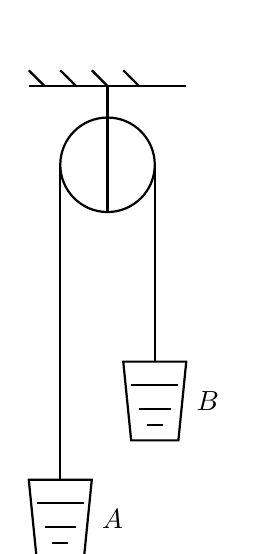
\begin{tikzpicture}[>=Stealth, thick]
    % Ceiling
    \draw (-1, 4) -- (1, 4);
    \foreach \x in {-0.8, -0.4, ..., 0.8} \draw (\x, 4) -- (\x-0.2, 4.2);
    
    % Pulley
    \draw (0, 4) -- (0, 3);
    \draw (0, 3) circle (0.6);
    \draw (0, 3) -- (0, 2.4); % center dot/line
    
    % Strings
    \draw (-0.6, 3) -- (-0.6, -1);
    \draw (0.6, 3) -- (0.6, 0.5);
    
    % Bucket A
    \draw (-1.0, -1) -- (-0.2, -1) -- (-0.3, -2) -- (-0.9, -2) -- cycle;
    \node[right] at (-0.2, -1.5) {$A$};
    % Water lines inside A
    \draw (-0.9, -1.3) -- (-0.3, -1.3);
    \draw (-0.8, -1.6) -- (-0.4, -1.6);
    \draw (-0.7, -1.8) -- (-0.5, -1.8);
    % Bucket A bottom hook/detail
    \draw (-0.6, -2) -- (-0.6, -2.1);
    
    % Bucket B
    \draw (0.2, 0.5) -- (1.0, 0.5) -- (0.9, -0.5) -- (0.3, -0.5) -- cycle;
    \node[right] at (1.0, 0) {$B$};
    % Water lines inside B
    \draw (0.3, 0.2) -- (0.9, 0.2);
    \draw (0.4, -0.1) -- (0.8, -0.1);
    \draw (0.5, -0.3) -- (0.7, -0.3);
\end{tikzpicture}}\\[4pt]
{\small 图 2-51（题 2-22）}
\end{center}

\newpage

\pdfbookmark[1]{题 2-23}{prob2-23}
\textbf{2-23} 系统如图 2-52 所示, 滑轮与细绳的质量均可略, 绳不可伸长. 设系统所有部位都没有摩擦, 物体 $B$ 借助于固定在大滑块 $C$ 右侧的导轨被限定沿 $C$ 的右侧面运动, 试求大滑块 $C$ 的运动加速度 $a_{c}$ .

\begin{center}
\resizebox{0.48\textwidth}{!}{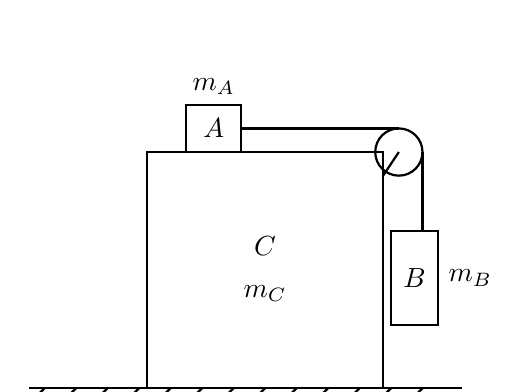
\begin{tikzpicture}[>=Stealth, thick]
    % Ground
    \draw (-1.5, 0) -- (4, 0);
    \foreach \x in {-1.3, -0.9, ..., 3.9} \draw (\x, 0) -- (\x-0.2, -0.2);
    
    % Block C
    \draw (0, 0) rectangle (3, 3);
    \node at (1.5, 1.8) {$C$};
    \node at (1.5, 1.2) {$m_C$};
    
    % Block A
    \draw (0.5, 3) rectangle (1.2, 3.6);
    \node at (0.85, 3.3) {$A$};
    \node[above] at (0.85, 3.6) {$m_A$};
    
    % Pulley
    \coordinate (P) at (3.2, 3);
    \draw (P) circle (0.3);
    \draw (3, 2.7) -- (P); % Bracket
    
    % Block B
    \draw (3.1, 0.8) rectangle (3.7, 2.0);
    \node at (3.4, 1.4) {$B$};
    \node[right] at (3.7, 1.4) {$m_B$};
    % Dashed line on the left side of B
    \draw[dashed] (3.0, 0.8) -- (3.0, 2.0); % The image has a dashed line between B and C. Actually C wall is at x=3.
    % So maybe B is at x=3.
    
    % Strings
    \draw (1.2, 3.3) -- (3.2, 3.3);
    \draw (3.5, 3) -- (3.5, 2.0);
\end{tikzpicture}}\\[4pt]
{\small 图 2-52（题 2-23）}
\end{center}

\newpage

\pdfbookmark[1]{题 2-24}{prob2-24}
\textbf{2-24} 如图 2-53 所示, $xy$ 平面是一绝缘水平面, $z$ 轴竖直向上, 在 $A(x_0,0,0)$ 处放置一电量为 $-q < 0$ , 质量可略的小物块, 物块与水平面间的摩擦因数为 $\mu$ , 物块与一细线相连, 细线的另一端 $B$ 穿过位于坐标原点 $O$ 的光滑小孔, 在水平面下方. 空间加一匀强电场, 场强 $E$ 的方向垂直于 $x$ 轴, 与 $z$ 轴夹角为 $\theta < \pi / 2$ , 且有 $\mu = \tan \theta$ . 今竖直向下缓慢拉动细线 $B$ 端, 使物块在水平面上移动过程的任一位置都可近似认为物块处于力平衡状态. 已知物块的移动轨迹是一条圆锥曲线, 试求其轨迹方程. (物块在电场中受力为 $F = -qE$ .)

\begin{center}
\resizebox{0.48\textwidth}{!}{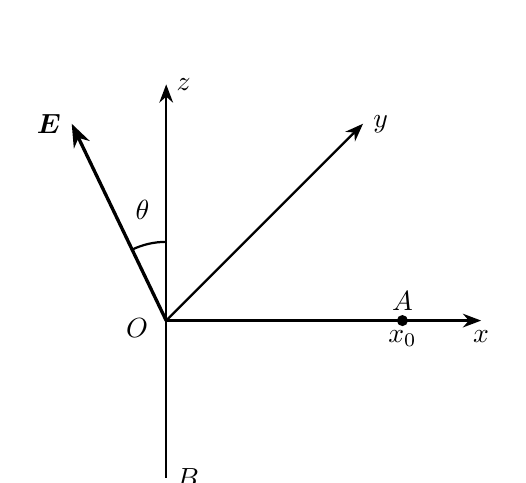
\begin{tikzpicture}[>=Stealth, thick]
    % Origin
    \coordinate (O) at (0, 0);
    \node[left] at (-0.1, -0.1) {$O$};
    
    % Axes
    \draw[->] (O) -- (4, 0) node[below] {$x$};
    \draw[->] (O) -- (2.5, 2.5) node[right] {$y$};
    \draw[->] (O) -- (0, 3) node[right] {$z$};
    
    % Vector E
    \draw[->, very thick] (O) -- (-1.2, 2.5) node[left] {$\boldsymbol{E}$};
    
    % Angle \theta
    \draw (0, 1) arc[start angle=90, end angle=115.6, radius=1]; % arctan(1.2/2.5) = 25.6, so 90 to 115.6
    \node at (-0.3, 1.4) {$\theta$};
    
    % Point A
    \fill (3, 0) circle (2pt) node[above] {$A$} node[below] {$x_0$};
    
    % Point B
    \draw (O) -- (0, -2) node[right] {$B$};
\end{tikzpicture}}\\[4pt]
{\small 图 2-53（题 2-24）}
\end{center}

\newpage

\pdfbookmark[1]{题 2-25}{prob2-25}
\textbf{2-25} 如图 2-54 所示, 平而薄的匀质圆板放在水平桌面上, 圆板绕着过中心 $O$ 的竖直轴旋转, $O$ 点沿桌面运动. 如果圆板与桌面间的摩擦因数处处相同, 试证圆板所受合摩擦力的方向必与 $O$ 点运动方向相反.

\begin{center}
\resizebox{0.32\textwidth}{!}{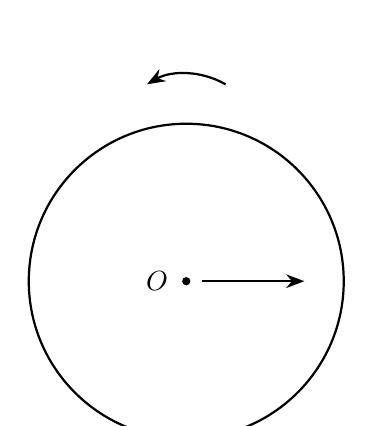
\begin{tikzpicture}[>=Stealth, thick]
    % Circle
    \draw (0, 0) circle (2);
    
    % Center O
    \fill (0, 0) circle (1.5pt);
    \node[left] at (-0.1, 0) {$O$};
    
    % Arrow right
    \draw[->] (0.2, 0) -- (1.5, 0);
    
    % Curved arrow top
    \draw[->] (0.5, 2.5) arc[start angle=60, end angle=120, radius=1.0];
\end{tikzpicture}}\\[4pt]
{\small 图 2-54（题 2-25）}
\end{center}

\newpage

\pdfbookmark[1]{题 2-26}{prob2-26}
\textbf{2-26} 质量同为 $m$ 的两个小球, 各自在空气中以速率 $v$ 运动时所受阻力大小为 $f = \alpha mv$ , 其中 $\alpha$ 是一个常量. 使两球位于同一竖直线上, 球 1 在球 2 上方 $h$ 处, 球 2 离地足够高, 在自由释放球 1 的同时, 以初速度 $v_0$ 将球 2 竖直向上抛出. 试问经多长时间 $t_0$ , 两球相遇?

\newpage

\pdfbookmark[1]{题 2-27}{prob2-27}
\textbf{2-27} 在静止的车厢内有一辐角为 $\theta (0 < \theta < 90^{\circ})$ 的圆锥摆，当摆球处于图 2-55 的最左位置时车厢开始以常量 $a$ 向右作水平匀加速运动.试问摆球相对车厢能否恰好从此时刻开始，以某 $\theta^{\prime}(0 < \theta^{\prime} < 90^{\circ})$ 为辐角作圆锥摆运动？

\begin{center}
\resizebox{0.47\textwidth}{!}{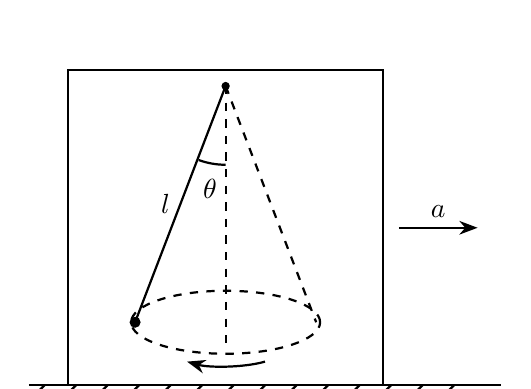
\begin{tikzpicture}[>=Stealth, thick]
    % Ground
    \draw (-2.5, 0) -- (3.5, 0);
    \foreach \x in {-2.3, -1.9, ..., 3.3} \draw (\x, 0) -- (\x-0.2, -0.2);
    
    % Box
    \draw (-2, 0) rectangle (2, 4);
    
    % Acceleration arrow
    \draw[->] (2.2, 2) -- (3.2, 2) node[midway, above] {$a$};
    
    % Conical Pendulum
    \coordinate (P) at (0, 3.8);
    \fill (P) circle (1.5pt);
    
    % Center line
    \draw[dashed] (P) -- (0, 0.5);
    
    % Base circle
    \draw[dashed] (0, 0.8) ellipse (1.2 and 0.4);
    
    % Pendulum string and mass
    \draw (P) -- (-1.15, 0.8) node[midway, left] {$l$};
    \fill (-1.15, 0.8) circle (2pt);
    
    % Dashed right string
    \draw[dashed] (P) -- (1.15, 0.8);
    
    % Angle \theta
    \draw (0, 2.8) arc[start angle=270, end angle=250, radius=1.0];
    \node at (-0.2, 2.5) {$\theta$};
    
    % Curved arrow at bottom
    \draw[->] (0.5, 0.3) arc[start angle=-45, end angle=-135, radius=0.7, y radius=0.2];
\end{tikzpicture}}\\[4pt]
{\small 图 2-55（题 2-27）}
\end{center}

\newpage

\pdfbookmark[1]{题 2-28}{prob2-28}
\textbf{2-28} 盛满同种液体的大容器以恒定的角速度 $\omega$ 绕着一固定轴旋转, 稳定后设液体密度 $\rho_{0}$ 仍可近似认为处处相同.

(1)如图 2-56 所示，在容器中以转轴与某旋转平面交点为坐标原点，设置径向坐标轴 $x$ ，沿 $x$ 方向取一细长条液柱，它的两端坐标分别为 $x_{1}$ 和 $x_{2}$ ，并且 $x_{2} > x_{1} \gg (x_{2} - x_{1})$ ，截面积同为 $S$ ，试求此液柱所受离心力 $\pmb{F}_{\mathrm{c}}$

(2) 不计重力, 计算 $x$ 处液体压强 $p(x)$ ;

(3) 将图 2-56 中的细液柱置换为外加的固态或液态细柱体, 不计重力, 计算它受到的 $\rho_{0}$ 液体施加的浮力 $F$.

\begin{center}
\resizebox{0.50\textwidth}{!}{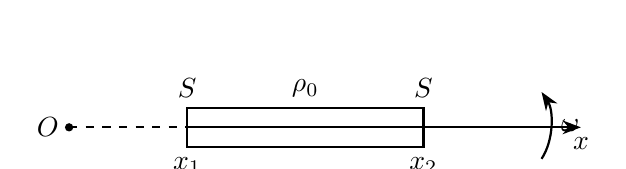
\begin{tikzpicture}[>=Stealth, thick]
    % Origin O
    \coordinate (O) at (0, 0);
    \fill (O) circle (1.5pt) node[left] {$O$};
    
    % Dashed axis
    \draw[dashed] (O) -- (1.5, 0);
    
    % Rod (Rectangle)
    \draw (1.5, -0.25) rectangle (4.5, 0.25);
    
    % Solid axis through rod
    \draw (1.5, 0) -- (4.5, 0);
    
    % Extending x-axis
    \draw[->] (4.5, 0) -- (6.5, 0) node[below] {$x$};
    
    % Labels
    \node[below] at (1.5, -0.25) {$x_1$};
    \node[below] at (4.5, -0.25) {$x_2$};
    \node[above] at (1.5, 0.25) {$S$};
    \node[above] at (4.5, 0.25) {$S$};
    \node[above] at (3.0, 0.25) {$\rho_0$};
    
    % Rotation arrow
    \draw[->] (6.0, -0.4) arc[start angle=-45, end angle=45, x radius=0.4, y radius=0.6] node[midway, right] {$\omega$};
\end{tikzpicture}}\\[4pt]
{\small 图 2-56（题 2-28）}
\end{center}

\newpage

\pdfbookmark[1]{题 2-29}{prob2-29}
\textbf{2-29} 如图 2-57 所示, 质量 $m_{1}$ 的航天飞机 $A$ 绕地球作匀速圆周运动, 轨道半径 $R$ , 从航天飞机伸出长 $L \ll R$ 的刚性杆, 杆端固定质量 $m_{2} \ll m_{1}$ 的卫星 $S$ . $A-S$ 系统的位置用 $\alpha$ 角表示, $\alpha$ 是杆与 $A$ 和地心连线之间的夹角. 试求 $A-S$ 系统的平衡位置, 并讨论平衡的稳定性. (稍偏离平衡位置, 静态下若有返回趋势者称为稳定平衡, 有远离趋势者称为不稳定平衡, 能停留者称为随遇平衡.)

\begin{center}
\resizebox{0.46\textwidth}{!}{\begin{tikzpicture}[>=Stealth, thick]
    % Earth surface arc
    \draw (-3.0, -3.5) to[out=15, in=165] (3.0, -3.5);
    
    % Mass A
    \coordinate (A) at (0, 0);
    \draw[pattern=north east lines] (A) circle (0.2);
    \draw (A) circle (0.2);
    \node[above] at (A) {$A$};
    \node[right] at (0.2, 0) {$m_1$};
    
    % Horizontal line and velocity v
    \draw (-0.2, 0) -- (-2.0, 0);
    \draw[->] (-0.2, 0) -- (-1.2, 0) node[above] {$v$};
    
    % Vertical R arrow
    \draw[->] (-1.6, 0) -- (-1.6, -4.0) node[midway, right] {$R$};
    \draw (-1.8, 0) -- (-1.4, 0); % Top tick mark for R
    
    % Vertical dashed line to earth center
    \draw[dashed, ->] (0, -0.2) -- (0, -4.5) node[below] {至地心};
    
    % Mass S and Rod L
    \coordinate (S) at (1.2, -2.0);
    \draw (0.1, -0.17) -- (S) node[midway, right] {$L$}; % start slightly offset from edge of A
    \fill (S) circle (1.5pt);
    \node[below] at (S) {$S$};
    \node[right] at (1.3, -2.0) {$m_2$};
    
    % Angle \alpha
    \draw (0, -0.8) arc[start angle=270, end angle=300.96, radius=0.8]; % arctan(1.2/2) = 30.96 deg
    \node at (0.25, -1.0) {$\alpha$};
\end{tikzpicture}}\\[4pt]
{\small 图 2-57（题 2-29）}
\end{center}

\newpage

\pdfbookmark[1]{题 2-30}{prob2-30}
\textbf{2-30} 不计空气阻力, 近似计算小球从北半球纬度 $\psi$ 上空 $h$ 处自由下落 ( $h \ll R$ (地球半径)), 因受科里奥利力影响产生的落地偏移值.

\newpage

\pdfbookmark[1]{题 2-31}{prob2-31}
\textbf{2-31} 如图 2-58 所示, 四个质量同为 $m$ 的小球, 用长度相同且不可伸长的轻绳连结成菱形 $ABCD$ , 静放在光滑的水平面上. 今突然给小球 $A$ 一个历时极短沿 $CA$ 方向的冲击, 使 $A$ 获得速度 $v$ . 已知 $\angle BAD = 2\alpha \left( \alpha < \frac{\pi}{4} \right)$ , 试求系统受冲击后瞬间具有的动量 $p$ 以及 $B, C, D$ 球各自速度 $v_B, v_C, v_D$ .

\begin{center}
\resizebox{0.49\textwidth}{!}{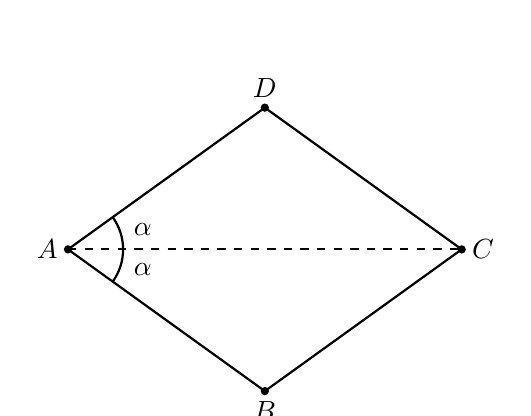
\begin{tikzpicture}[>=Stealth, thick]
    \coordinate (A) at (-2.5, 0);
    \coordinate (B) at (0, -1.8);
    \coordinate (C) at (2.5, 0);
    \coordinate (D) at (0, 1.8);

    \draw (A) -- (B) -- (C) -- (D) -- cycle;
    \draw[dashed] (A) -- (C);

    \fill (A) circle (1.5pt) node[left] {$A$};
    \fill (B) circle (1.5pt) node[below] {$B$};
    \fill (C) circle (1.5pt) node[right] {$C$};
    \fill (D) circle (1.5pt) node[above] {$D$};

    % Angle \alpha
    % arctan(1.8/2.5) = 35.75 deg
    \draw (-1.8, 0) arc[start angle=0, end angle=35.75, radius=0.7];
    \node at (-1.55, 0.25) {$\alpha$};
    
    \draw (-1.8, 0) arc[start angle=0, end angle=-35.75, radius=0.7];
    \node at (-1.55, -0.25) {$\alpha$};
\end{tikzpicture}}\\[4pt]
{\small 图 2-58（题 2-31）}
\end{center}

\newpage

\pdfbookmark[1]{题 2-32}{prob2-32}
\textbf{2-32} 从地面发射的炮弹在达到最高点处炸裂成质量相同的两块, 第一块在炸裂后 1 $s$ 落到爆炸点正下方的地面上, 该处与发射点的距离为 $s_{1}=1000$ $m$. 已知最高点距地面高度 h=19.6 $m$, 忽略空气阻力,试求第二块的落地点与发射点的距离.

\newpage

\pdfbookmark[1]{题 2-33}{prob2-33}
\textbf{2-33} 船静止在水面上, 人从船的一端走到另一端, 再返回这一端, 若不计水的阻力, 船往返合成位移为零. 真实情况下水有阻力, 如果来回走的快慢不一样, 船就有可能获得非零的合成位移. 水的阻力较复杂, 可以改取水平地面上有摩擦的长木板, 板上的小物块替换人, 组合成较初等的题目.

如图 2-59 所示, 质量 M=3m, 长 2l 的均匀长木板静止在水平地面上, 两者间摩擦因数 $\mu=1/8$ . 板的右端有一质量 $m$ 的小物块, 从静止出发通过与木板的某种相互作用机制, 相对木板以朝左的恒定加速度 $a = \frac{1}{2}\alpha g$ 运动，其中 $\alpha > 1$ 是一个不变的参数。小物块到达板中央后，立即改成以 $a = \frac{1}{2}\alpha g$ 的反向加速度继续相对木板运动到左端停下，直到木板在地面上不再运动为止。

(1) 计算木板在地面上朝右的总位移大小 $s_{\text{右}}$ ;

(2) 若小物块再以同样方式从板的左端运动到板的右端, 只是将 $a$ 换成 $a' = \frac{1}{2} \alpha' g, \alpha' > 1$ , 导出此过程中木板朝左总位移大小 $s_{\text{左}}$ ;

(3) 小物块如上所述, 在木板上往返一次, 确定木板在地面上合成位移的方向和大小 $s$.

\begin{center}
\resizebox{0.50\textwidth}{!}{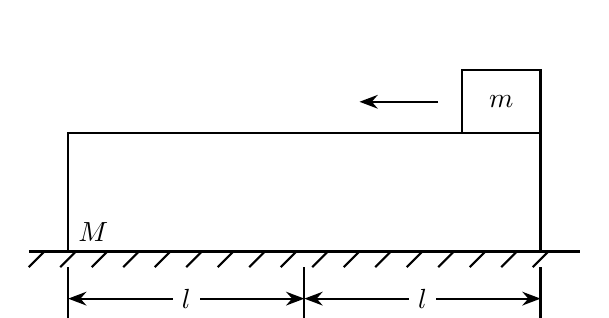
\begin{tikzpicture}[>=Stealth, thick]
    % Ground
    \draw (-3.5, 0) -- (3.5, 0);
    \foreach \x in {-3.3, -2.9, ..., 3.3} \draw (\x, 0) -- (\x-0.2, -0.2);

    % Block M
    \draw (-3, 0) rectangle (3, 1.5);
    \node[above right] at (-3, 0) {$M$};

    % Block m
    \draw (2, 1.5) rectangle (3, 2.3);
    \node at (2.5, 1.9) {$m$};

    % Arrow on m
    \draw[->, thick] (1.7, 1.9) -- (0.7, 1.9);

    % Dimension lines
    \draw (-3, -0.2) -- (-3, -1.0);
    \draw (0, -0.2) -- (0, -1.0);
    \draw (3, -0.2) -- (3, -1.0);

    \draw[<->] (-3, -0.6) -- (0, -0.6) node[midway, fill=white] {$l$};
    \draw[<->] (0, -0.6) -- (3, -0.6) node[midway, fill=white] {$l$};
\end{tikzpicture}}\\[4pt]
{\small 图 2-59（题 2-33）}
\end{center}

\newpage

\pdfbookmark[1]{题 2-34}{prob2-34}
\textbf{2-34} 球状小水滴在静止的雾气中下落, 下落过程中吸附了全部所遇到的水分子. 设水滴始终保持球状, 雾气密度均匀, 略去空气的黏力, 重力加速度 $g$ 视为不变, 试证经过足够长时间后, 水滴下落加速度趋于稳定值, 并求出此值. 已知满足方程

\[
\frac {\mathrm{d} ^ {2} y}{\mathrm{d} x ^ {2}} + \frac {A}{y} \left(\frac {\mathrm{d} y}{\mathrm{d} x}\right) ^ {2} = B
\]

的函数 $y(x)$ ，其解为

\[
y = (C _ {1} x + C _ {2}) ^ {\frac {1}{A + 1}} + \frac {B}{2 (2 A + 1)} x ^ {2},
\]

其中 $C_1, C_2$ 是两个待定的积分常数.

% FIGSCALE 0.8 / BOOKMARKS
\chapter{机械能定理}

\pdfbookmark[1]{题 3-1}{prob3-1}
\textbf{3-1} 图 3-39 中的 $A_{3}BCD_{3}$ 是一条长轨道, 其中 $A_{3}B$ 是斜面段, $CD_{3}$ 是水平段, BC 是与 $A_{3}B$ 和 $CD_{3}$ 都相切的一小段圆弧. 一个小球与斜面段各处摩擦因数相同, 小球与水平段各处摩擦因数也都相同，但这两个摩擦因数未必相同。小球依次由 $A_{1}, A_{2}, A_{3}$ 从静止开始滑下，最后分别停留在 $D_{1}, D_{2}, D_{3}$ 点。已知 $h_{2} - h_{1} = 0.30 \mathrm{~m}, h_{3} - h_{2} = 0.48 \mathrm{~m}, \overline{D_{1} D_{2}} = 1.5 \mathrm{~m}$ ，试求 $\overline{D_{2} D_{3}}$ 长度。

\begin{center}
\resizebox{0.50\textwidth}{!}{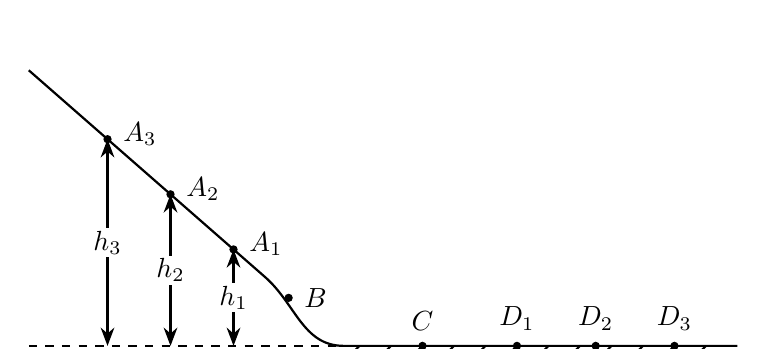
\begin{tikzpicture}[>=Stealth, thick]
    % 定义斜面和水平面的关键坐标
    \coordinate (Start) at (-1, 3.5);
    \coordinate (CurveStart) at (2, 0.875); % 斜率设为 -0.875
    \coordinate (CurveEnd) at (3, 0);
    \coordinate (GroundEnd) at (8, 0);
    
    % 绘制斜面、圆滑过渡段和水平面
    \draw (Start) -- (CurveStart) to[out=-41.2, in=180] (CurveEnd) -- (GroundEnd);
    
    % 绘制斜面下方的虚线辅助水平线
    \draw[dashed] (-1, 0) -- (3, 0);
    
    % 绘制水平面下的阴影线
    \foreach \x in {3.2, 3.6, ..., 7.8} {
        \draw (\x, 0) -- (\x-0.2, -0.2);
    }
    
    % 选取斜面上的点 A3, A2, A1 (保证在直线上)
    \coordinate (A3) at (0, 2.625);
    \coordinate (A2) at (0.8, 1.925);
    \coordinate (A1) at (1.6, 1.225);
    
    % 绘制点并标注
    \fill (A3) circle (1.5pt) node[right=2pt, yshift=2pt] {$A_3$};
    \fill (A2) circle (1.5pt) node[right=2pt, yshift=2pt] {$A_2$};
    \fill (A1) circle (1.5pt) node[right=2pt, yshift=2pt] {$A_1$};
    
    % 绘制高度标注箭头
    \draw[<->] (0, 0) -- (A3) node[midway, fill=white, inner sep=1pt] {$h_3$};
    \draw[<->] (0.8, 0) -- (A2) node[midway, fill=white, inner sep=1pt] {$h_2$};
    \draw[<->] (1.6, 0) -- (A1) node[midway, fill=white, inner sep=1pt] {$h_1$};
    
    % B点 (过渡曲线附近)
    \coordinate (B) at (2.3, 0.61);
    \fill (B) circle (1.5pt) node[right=2pt] {$B$};
    
    % 水平面上的点 C, D1, D2, D3
    \fill (4, 0) circle (1.5pt) node[above=2pt] {$C$};
    \fill (5.2, 0) circle (1.5pt) node[above=2pt] {$D_1$};
    \fill (6.2, 0) circle (1.5pt) node[above=2pt] {$D_2$};
    \fill (7.2, 0) circle (1.5pt) node[above=2pt] {$D_3$};
\end{tikzpicture}}\\[4pt]
{\small 图 3-39（题 3-1）}
\end{center}

\newpage

\pdfbookmark[1]{题 3-2}{prob3-2}
\textbf{3-2} 某人心脏每搏动一次泵出 80.0 mL 的血液, 一次搏动过程中心脏主动脉平均压强为 120 mmHg. 已知此人脉搏为 70.0 次/min, 试求此人心脏工作的功率.

\newpage

\pdfbookmark[1]{题 3-3}{prob3-3}
\textbf{3-3} 质量同为 $m$ 的两个小球, 用长 $2l$ 轻绳连接后静放在光滑水平面上, 绳处于伸直状态, 如图 3-40 所示. 今用恒力 $\pmb{F}$ 作用于绳的中央, $\pmb{F}$ 方向水平且垂直于绳的初始长度方向, 两球因此运动. 试问在两球第一次相碰前的瞬间, 小球在垂直于 $\pmb{F}$ 作用线方向上的分速度 $v_{\perp}$ 为多大?

\begin{center}
\resizebox{0.21\textwidth}{!}{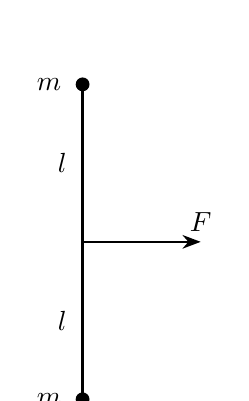
\begin{tikzpicture}[>=Stealth, thick]
    % 杆的上下端点及中心
    \coordinate (Top) at (0, 2);
    \coordinate (Bot) at (0, -2);
    \coordinate (Mid) at (0, 0);
    
    % 绘制细杆
    \draw (Top) -- (Bot);
    
    % 绘制两端的质点并标注 m
    \fill (Top) circle (2.5pt) node[left=4pt] {$m$};
    \fill (Bot) circle (2.5pt) node[left=4pt] {$m$};
    
    % 标注长度 l
    \node[left=2pt] at (0, 1) {$l$};
    \node[left=2pt] at (0, -1) {$l$};
    
    % 中间的受力箭头 F
    \draw[->, thick] (Mid) -- (1.5, 0) node[above] {$F$};
\end{tikzpicture}}\\[4pt]
{\small 图 3-40（题 3-3）}
\end{center}

\newpage

\pdfbookmark[1]{题 3-4}{prob3-4}
\textbf{3-4} 如图 3-41 所示, 表面光滑, 高 $h$、倾角 $\phi$ 的劈形物块以恒定速度 $u$ 水平朝右运动, 在其斜面顶端有一个质量 $m$ 的小木块从相对静止状态开始滑到底端.

(1) 计算小木块相对劈形物块的末速度大小 $v'$ ;

(2) 在地面系计算小木块动能总增量 $\Delta E_{k}$ ;

(3) 在地面系计算斜面支持力 $N$ 对小木块所作总功 $W_{N}$ ;

(4)在地面系验证 $W_{N} + W_{g} = \Delta E_{k}$ ，其中 $W_{g}$ 是重力对小木块所作总功.

\begin{center}
\resizebox{0.50\textwidth}{!}{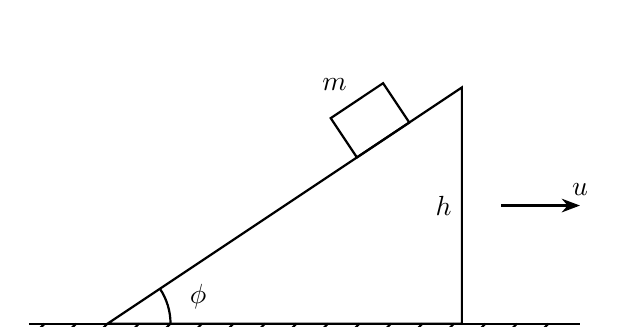
\begin{tikzpicture}[>=Stealth, thick]
    % 地面及阴影线
    \draw (-1, 0) -- (6, 0);
    \foreach \x in {-0.8, -0.4, ..., 5.8} {
        \draw (\x, 0) -- (\x-0.2, -0.2);
    }
    
    % 斜面 (三角形)
    \coordinate (O) at (0, 0);
    \coordinate (R) at (4.5, 0);
    \coordinate (T) at (4.5, 3);
    \draw (O) -- (R) -- (T) -- cycle;
    
    % 角度 \phi
    % 角度计算: arctan(3/4.5) ≈ 33.7°
    \draw (0.8, 0) arc[start angle=0, end angle=33.7, radius=0.8];
    \node at (1.15, 0.35) {$\phi$};
    
    % 高度标注 h
    \node[left] at (4.5, 1.5) {$h$};
    
    % 斜面整体移动的速度 u
    \draw[->, thick] (5.0, 1.5) -- (6.0, 1.5) node[above] {$u$};
    
    % 斜面上的滑块 m
    \begin{scope}[shift={(3.5, 2.333)}, rotate=33.7]
        \draw[thick] (-0.4, 0) rectangle (0.4, 0.6);
        \node[above left] at (0, 0.6) {$m$};
    \end{scope}
\end{tikzpicture}}\\[4pt]
{\small 图 3-41（题 3-4）}
\end{center}

\newpage

\pdfbookmark[1]{题 3-5}{prob3-5}
\textbf{3-5} 两个仅可压缩的轻弹簧组成的水平弹簧组如图 3-42 所示, 弹簧 1 和 2 的劲度系数分别为 $k_{1}$ 和 $k_{2}$ , 它们的自由长度相差 $l$ . 建立图示的 $x$ 轴, 原点位于弹簧 2 的自由端, 图中长挡板的位置记为 $x$ . 系统势能 $E_{\mathrm{p}}(x)$ 零点按下述两种方式设定, 分别在 $0 \leqslant x \leqslant l$ 和 $x < 0$ 两个范围导出 $E_{\mathrm{p}}(x) - x$ 关系式: 

(1) 设定 $x = 0$ 点为系统势能零点; 

(2) 设定 $x = l$ 点为系统势能零点.

\begin{center}
\resizebox{0.50\textwidth}{!}{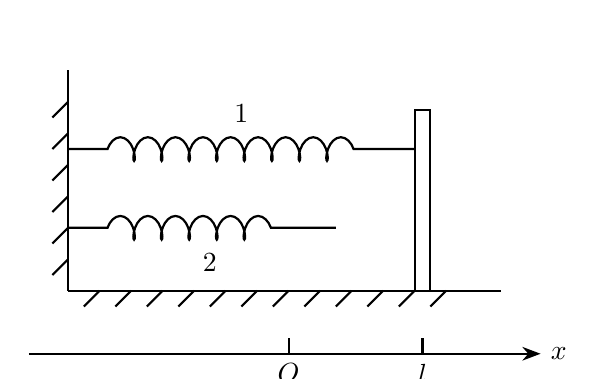
\begin{tikzpicture}[>=Stealth, thick]
    % 竖直墙面及阴影
    \draw (0, 0) -- (0, 2.8);
    \foreach \y in {0.4, 0.8, ..., 2.8} {
        \draw (0, \y) -- (-0.2, \y-0.2);
    }
    
    % 水平地面及阴影
    \draw (0, 0) -- (5.5, 0);
    \foreach \x in {0.4, 0.8, ..., 5.2} {
        \draw (\x, 0) -- (\x-0.2, -0.2);
    }
    
    % 挡板 (空心矩形)
    \draw[fill=white, thick] (4.4, 0) rectangle (4.6, 2.3);
    
    % 弹簧 1 (使用 coil 装饰器自动生成弹簧圈，设置前后平直长度为5mm)
    \draw[decorate, decoration={coil, aspect=0.5, segment length=3.5mm, amplitude=1.5mm, pre length=5mm, post length=5mm}] 
        (0, 1.8) -- (4.4, 1.8);
    \node[above] at (2.2, 2.0) {1};
    
    % 弹簧 2
    \draw[decorate, decoration={coil, aspect=0.5, segment length=3.5mm, amplitude=1.5mm, pre length=5mm, post length=5mm}] 
        (0, 0.8) -- (3.4, 0.8);
    \node[below] at (1.8, 0.6) {2};
    
    % 下方的 x 坐标轴及标记
    \draw[->] (-0.5, -0.8) -- (6.0, -0.8) node[right] {$x$};
    
    % 原点 O 标记
    \draw (2.8, -0.8) -- (2.8, -0.6);
    \node[below] at (2.8, -0.8) {$O$};
    
    % 挡板位置 l 标记
    \draw (4.5, -0.8) -- (4.5, -0.6);
    \node[below] at (4.5, -0.8) {$l$};
\end{tikzpicture}}\\[4pt]
{\small 图 3-42（题 3-5）}
\end{center}

\newpage

\pdfbookmark[1]{题 3-6}{prob3-6}
\textbf{3-6} 地震的里氏(Richter)震级 $M$ 与从其释放出来的能量 $E$ 之间的关系为
\[
\log E = 5. 2 4 + 1. 4 4 M,
\]
式中 $E$ 的单位为 $J$. 1679 年 9 月 2 日, 北京地区发生过一次 8 级地震, 试求该次地震释放的能量.

长江源头为青海高原昆仑山南麓的沱沱河，从这里经 $5000\mathrm{m}$ 落差注入东海，它的水利资源的储存量按功率计为 $1.125 \times 10^{8} \mathrm{kW}$ . 试比较长江一天内所提供的水利资源能量与上述地震释放的能量哪一个大？估算长江的平均流量.

\newpage

\pdfbookmark[1]{题 3-7}{prob3-7}
\textbf{3-7} 杂技演员站在蹦床上不动时,网下沉 0.20 $m$,试问当演员从 10.0 $m$ 高处自由下落时,蹦床网将受到的最大压力是杂技演员自身重力的多少倍(给出 3 位有效数字)?已知网的下沉量与正压力的二次方根成正比.

\newpage

\pdfbookmark[1]{题 3-8}{prob3-8}
\textbf{3-8} 如图 3-43 所示, 用细绳悬挂一个匀质圆环, 环上穿两个质量相同的小串珠, 小串珠与环之间无摩擦. 令小串珠从环顶左、右两侧自静止开始自由滑下, 为使过程中环会上升, 试求环的质量与一个小串珠的质量之比 $\gamma$ 的可取值.

\begin{center}
\resizebox{0.34\textwidth}{!}{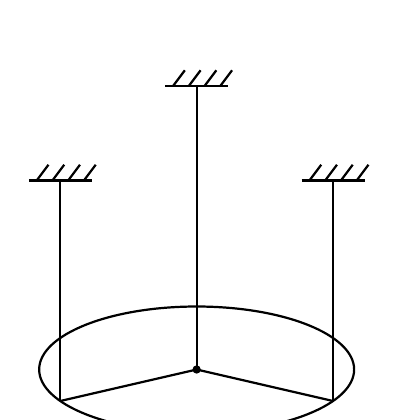
\begin{tikzpicture}[>=Stealth, thick]
    % 定义椭圆环
    \draw (0, 0) ellipse (2cm and 0.8cm);
    
    % 中心交点
    \fill (0, 0) circle (1.5pt);
    
    % 定义圆环上的三个附着点 (约 90°, 210°, 330°)
    \coordinate (P1) at (0, 0.8);
    \coordinate (P2) at (-1.732, -0.4);
    \coordinate (P3) at (1.732, -0.4);
    
    % 从中心到附着点的径向连线
    \draw (0, 0) -- (P1);
    \draw (0, 0) -- (P2);
    \draw (0, 0) -- (P3);
    
    % 竖直悬挂线
    \draw (P1) -- ++(0, 2.8) coordinate (C1);
    \draw (P2) -- ++(0, 2.8) coordinate (C2);
    \draw (P3) -- ++(0, 2.8) coordinate (C3);
    
    % 绘制天花板固定端及其阴影线
    \foreach \P in {C1, C2, C3} {
        \draw (\P) +(-0.4, 0) -- +(0.4, 0);
        \foreach \x in {-0.3, -0.1, 0.1, 0.3} {
            \draw (\P) +(\x, 0) -- +(\x+0.15, 0.2);
        }
    }
\end{tikzpicture}}\\[4pt]
{\small 图 3-43（题 3-8）}
\end{center}

\newpage

\pdfbookmark[1]{题 3-9}{prob3-9}
\textbf{3-9} 大质量车厢在水平地面上以 $v_{0}$ 速度匀速行使, 车厢内有一半径 $R$ 的光滑半圆柱面, 顶部有一质量为 $m$ 的小球. 开始时小球静止, 如图 3-44 所示, 而后因微小扰动下滑离开圆柱面, 试求过程中圆柱面支持力 $N$ 对小球所作功.

\begin{center}
\resizebox{0.50\textwidth}{!}{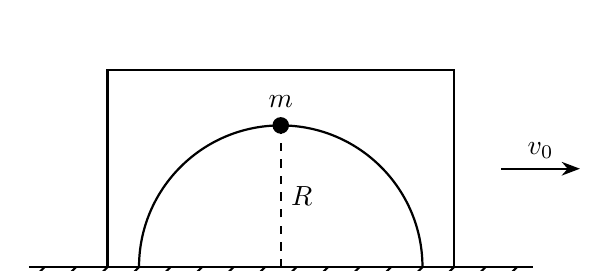
\begin{tikzpicture}[>=Stealth, thick]
    % 地面及阴影线
    \draw (-3.2, 0) -- (3.2, 0);
    \foreach \x in {-3.0, -2.6, ..., 3.0} {
        \draw (\x, 0) -- (\x-0.2, -0.2);
    }
    
    % 外部方块
    \draw (-2.2, 0) -- (-2.2, 2.5) -- (2.2, 2.5) -- (2.2, 0);
    
    % 半圆形凹槽
    \draw (1.8, 0) arc[start angle=0, end angle=180, radius=1.8];
    
    % 顶部的质点 m
    \fill (0, 1.8) circle (3pt);
    \node[above] at (0, 1.9) {$m$};
    
    % 半径 R 及虚线
    \draw[dashed] (0, 0) -- (0, 1.8);
    \node[right] at (0, 0.9) {$R$};
    
    % 整体向右的速度 v_0
    \draw[->] (2.8, 1.25) -- (3.8, 1.25) node[midway, above] {$v_0$};
\end{tikzpicture}}\\[4pt]
{\small 图 3-44（题 3-9）}
\end{center}

\newpage

\pdfbookmark[1]{题 3-10}{prob3-10}
\textbf{3-10} 用三根等长轻线, 将质量均匀分布的圆环对称地悬挂在天花板下, 构成一个扭摆, 小角度扭转周期为 $T_{0}$ . 再用三根轻质辐条在圆环中心固定一个与环质量相同的小物块, 如图 3-45 所示, 保持扭转幅度相同, 新系统扭转周期记为 $T$ , 试求 $T$ 与 $T_{0}$ 的比值 $\gamma$ .

\begin{center}
\resizebox{0.32\textwidth}{!}{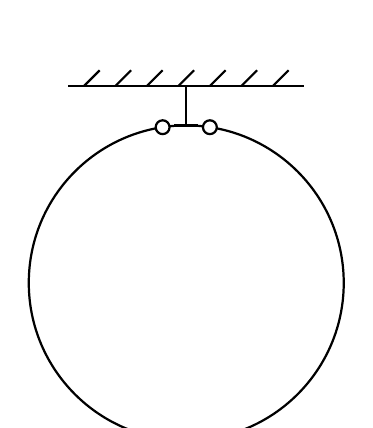
\begin{tikzpicture}[>=Stealth, thick]
    % 天花板
    \draw (-1.5, 3) -- (1.5, 3);
    \foreach \x in {-1.3, -0.9, ..., 1.3} {
        \draw (\x, 3) -- (\x+0.2, 3.2);
    }
    
    % 竖直悬挂线及底部小横杆
    \draw (0, 3) -- (0, 2.5);
    \draw (-0.15, 2.5) -- (0.15, 2.5);
    
    % 大圆环
    \draw (0, 0.5) circle (2cm);
    
    % 顶部的两个空心小珠子 (位于连接点两侧)
    \draw[fill=white, thick] (-0.3, 2.477) circle (2.5pt);
    \draw[fill=white, thick] (0.3, 2.477) circle (2.5pt);
\end{tikzpicture}}\\[4pt]
{\small 图 3-45（题 3-10）}
\end{center}

\newpage

\pdfbookmark[1]{题 3-11}{prob3-11}
\textbf{3-11} 系统如图 3-46 所示, $A$ 和 $B$ 是两个质量相同的小球, 其间是一根轻杆, 竖直线代表竖直光滑墙, 水平线代表水平光滑地面, 开始时 $\theta = 0$ , $A$, $B$ 及杆静止, 而后因微小扰动而下滑, 试问 $\theta$ 达到何值时 $A$ 球离墙?

\begin{center}
\resizebox{0.37\textwidth}{!}{\begin{tikzpicture}[>=Stealth, thick]
    % 竖直墙面和水平地面
    \draw (0, 4) -- (0, 0) -- (4.5, 0);
    
    % 杆 AB
    \coordinate (A) at (0, 3.5);
    \coordinate (B) at (2.8, 0);
    \draw (A) -- (B);
    
    % 端点 A 和 B
    \fill (A) circle (2pt) node[right, xshift=2pt] {$A$};
    \fill (B) circle (2pt) node[above right] {$B$};
    
    % 夹角 \theta
    % arctan(2.8/3.5) ≈ 38.66° -> 取相对垂直方向的圆弧
    \draw (0, 2.5) arc[start angle=270, end angle=308.6, radius=1];
    \node at (0.3, 2.1) {$\theta$};
\end{tikzpicture}}\\[4pt]
{\small 图 3-46（题 3-11）}
\end{center}

\newpage

\pdfbookmark[1]{题 3-12}{prob3-12}
\textbf{3-12} 系统如图 3-47 所示, 细绳的质量线密度为常量 $\lambda$ , 长 $\pi R + H$ , 其中 $\pi R$ 段搭在半径 $R$ 且固定不可转动的滑轮上, 绳与滑轮光滑接触. 绳左侧 $H$ 段的下端恰好与水平地面自由接触, 绳的右端连接质量 $m = \frac{1}{2} \lambda H$ 的小重物. 开始时系统处于运动状态, 小重物具有竖直向下的速度 $v_0$ , 绳中各部位也具有沿绳方向的速度 $v_0$ . 为使小重物能在滑轮右侧着地, 试求 $v_0$ . (假设已有图中未画出的装置, 使绳不会甩离滑轮.)

\begin{center}
\resizebox{0.36\textwidth}{!}{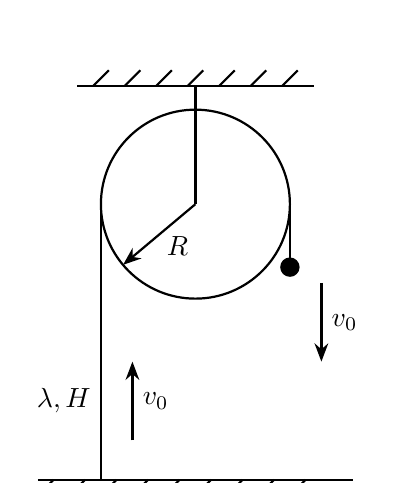
\begin{tikzpicture}[>=Stealth, thick]
    % 天花板
    \draw (-1.5, 3.5) -- (1.5, 3.5);
    \foreach \x in {-1.3, -0.9, ..., 1.3} {
        \draw (\x, 3.5) -- (\x+0.2, 3.7);
    }
    
    % 滑轮支架及滑轮
    \draw (0, 3.5) -- (0, 2);
    \draw (0, 2) circle (1.2cm);
    
    % 半径 R 标注 (已修复：添加了 ++ 相对坐标前缀)
    \draw[->] (0, 2) -- ++(220:1.2) node[midway, right, xshift=-1pt, yshift=-4pt] {$R$};
    
    % 地面
    \draw (-2, -1.5) -- (2, -1.5);
    \foreach \x in {-1.8, -1.4, ..., 1.8} {
        \draw (\x, -1.5) -- (\x-0.2, -1.7);
    }
    
    % 左侧链条(直线)与参数
    \draw (-1.2, 2) -- (-1.2, -1.5);
    \node[left] at (-1.2, -0.5) {$\lambda, H$};
    \draw[->] (-0.8, -1.0) -- (-0.8, 0.0) node[midway, right] {$v_0$};
    
    % 右侧线及质点
    \draw (1.2, 2) -- (1.2, 1.2);
    \fill (1.2, 1.2) circle (3.5pt);
    \draw[->] (1.6, 1.0) -- (1.6, 0.0) node[midway, right] {$v_0$};
\end{tikzpicture}}\\[4pt]
{\small 图 3-47（题 3-12）}
\end{center}

\newpage

\pdfbookmark[1]{题 3-13}{prob3-13}
\textbf{3-13} 如图 3-48 所示, 两个等高的小定滑轮相距 2 $m$, 物块 $A$ 和 $B$ 的质量各为 1 kg, 它们之间用轻绳连接, 在绳的水平段中点挂一个质量 1.9 kg 的小物块 $C$, 开始时均处于静止状态. 而后 $C$ 被释放, 三物块同时开始运动, 当 $C$ 下降 0.75 $m$ 时, 试问:

(1) $A$, $B$, $C$ 的速度各是多少?

(2) $A$, $B$, $C$ 的加速度各是多少?

\begin{center}
\resizebox{0.50\textwidth}{!}{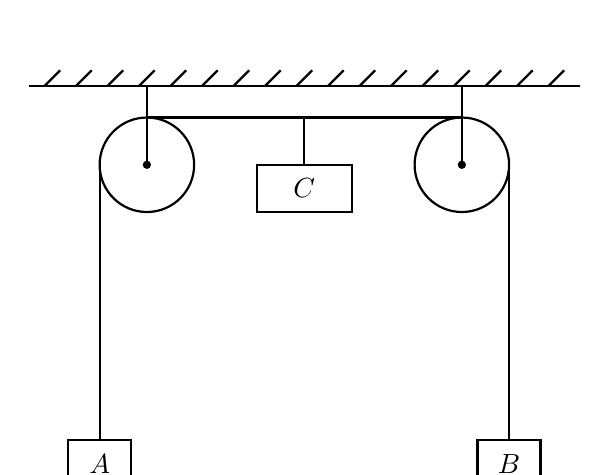
\begin{tikzpicture}[>=Stealth, thick]
    % 天花板
    \draw (-3.5, 3.5) -- (3.5, 3.5);
    \foreach \x in {-3.3, -2.9, ..., 3.3} {
        \draw (\x, 3.5) -- (\x+0.2, 3.7);
    }
    
    % 左右定滑轮
    \coordinate (P1) at (-2, 2.5);
    \coordinate (P2) at (2, 2.5);
    \draw (P1) circle (0.6);
    \draw (P2) circle (0.6);
    \fill (P1) circle (1.5pt);
    \fill (P2) circle (1.5pt);
    
    % 悬挂支架
    \draw (-2, 3.5) -- (P1);
    \draw (2, 3.5) -- (P2);
    
    % 连接三个物块的绳索
    \draw (-2.6, 2.5) -- (-2.6, -1); % 左垂线
    \draw (-2, 3.1) -- (2, 3.1);     % 滑轮间水平线 (与两圆顶部相切)
    \draw (2.6, 2.5) -- (2.6, -1);   % 右垂线
    
    % 中央悬挂绳
    \draw (0, 3.1) -- (0, 2.5);
    
    % 绘制物块 A, B, C
    \draw[thick, fill=white] (-3.0, -1.6) rectangle (-2.2, -1.0) node[midway] {$A$};
    \draw[thick, fill=white] (2.2, -1.6) rectangle (3.0, -1.0) node[midway] {$B$};
    \draw[thick, fill=white] (-0.6, 1.9) rectangle (0.6, 2.5) node[midway] {$C$};
\end{tikzpicture}}\\[4pt]
{\small 图 3-48（题 3-13）}
\end{center}

\newpage

\pdfbookmark[1]{题 3-14}{prob3-14}
\textbf{3-14} 如图 3-49 所示, 两根长度同为 $l$ 的轻杆用质量 $m$ 的球形铰链相接, 两杆另一端分别连接质量 $m$ 和 $2m$ 的小球. 开始时两杆并拢竖立在光滑水平面上, 铰链球在上, 而后从静止释放, 下面两球朝两侧滑动, 两杆始终在同一竖直平面内. 略去所有阻力, 试求:

(1) 铰链球碰到桌面时的速度；

(2) 两杆夹角为 $90^{\circ}$ 时, 质量为 2m 的小球速度.

\begin{center}
\resizebox{0.47\textwidth}{!}{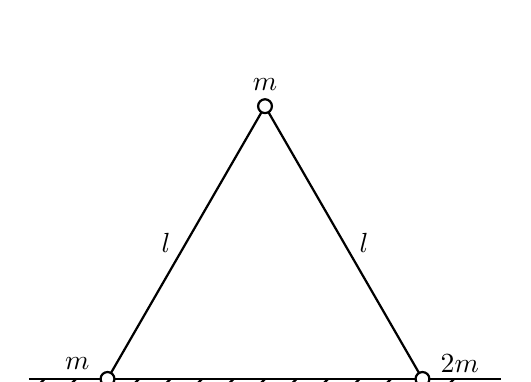
\begin{tikzpicture}[>=Stealth, thick]
    % 地面及阴影线
    \draw (-1, 0) -- (5, 0);
    \foreach \x in {-0.8, -0.4, ..., 4.8} {
        \draw (\x, 0) -- (\x-0.2, -0.2);
    }
    
    % 定义三个顶点 (等腰三角形结构)
    \coordinate (A) at (0, 0);
    \coordinate (B) at (4, 0);
    \coordinate (C) at (2, 3.464); % 4 * sin(60) ≈ 3.464
    
    % 绘制连杆
    \draw (A) -- (C) node[midway, left=2pt] {$l$};
    \draw (B) -- (C) node[midway, right=2pt] {$l$};
    
    % 绘制质点空心圆及标注
    \fill[white] (A) circle (2.5pt); \draw (A) circle (2.5pt);
    \fill[white] (B) circle (2.5pt); \draw (B) circle (2.5pt);
    \fill[white] (C) circle (2.5pt); \draw (C) circle (2.5pt);
    
    \node[left] at (-0.1, 0.2) {$m$};
    \node[right] at (4.1, 0.2) {$2m$};
    \node[above=2pt] at (C) {$m$};
\end{tikzpicture}}\\[4pt]
{\small 图 3-49（题 3-14）}
\end{center}

\newpage

\pdfbookmark[1]{题 3-15}{prob3-15}
\textbf{3-15} 一个足够深, 长 $l$ 、宽 $b$ 的矩形盛水鱼缸放在车厢内, 缸的长边方向与车厢长边方向一致. 火车匀速行进时, 水面与缸口相距 $h$ . 某时刻开始, 火车作加速度为常量 $a$ 的直线运动, 为使水不溢出, 求 $a$ 的最大可取值, 设缸中水面可近似处理为始终保持平面形状.

\newpage

\pdfbookmark[1]{题 3-16}{prob3-16}
\textbf{3-16} 核电站的原子能反应堆中需要用低速热中子维持缓慢的链式反应, 反应释放的却是高速快中子. 反应堆中通过快中子与石墨棒内碳原子 $\left(^{12}_{6}\mathrm{C}\right)$ 的不断碰撞逐渐减速，最后成为所需要的热中子。将快中子与热中子的平均动能分别设为 $2.0\times10^{6}eV$ 和 $0.025eV$ ，每次碰撞前碳原子均处于静止状态，碰撞为弹性。试问经过多少次碰撞，快中子可成为热中子？

\newpage

\pdfbookmark[1]{题 3-17}{prob3-17}
\textbf{3-17} “弹弓效应”是航天技术中增大宇宙探测器速率的一种有效方法. 如图 3-50 所示, 土星以相对于太阳的轨道速率 $v_{M}=9.6$ km/s 运行, 一空间探测器以相对于太阳的速率 $v_{0}=10.4$ km/s 迎向土星飞行. 由于土星的引力, 探测器绕过土星沿着和原来相反的方向离去,试求探测器离去时相对于太阳的速率 $v$.

\begin{center}
\resizebox{0.50\textwidth}{!}{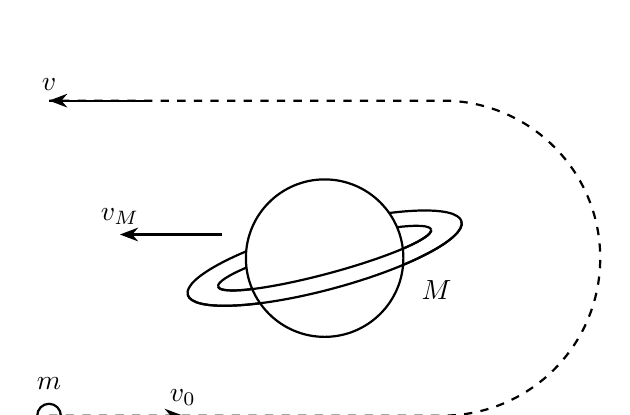
\begin{tikzpicture}[>=Stealth, thick]
    % 行星与星环
    \begin{scope}[rotate=15]
        % 星环后半部分 (被行星遮挡前先画)
        \draw (-1.8, 0) arc (180:360:1.8 and 0.4);
        \draw (-1.4, 0) arc (180:360:1.4 and 0.2);
        \draw (1.8, 0) arc (0:180:1.8 and 0.4);
        \draw (1.4, 0) arc (0:180:1.4 and 0.2);
    \end{scope}
    
    % 行星本体
    \fill[white] (0, 0) circle (1.0);
    \draw (0, 0) circle (1.0);
    \node[right] at (1.1, -0.4) {$M$};
    
    % 星环前半部分 (覆盖在行星上)
    \begin{scope}[rotate=15]
        \draw (-1.8, 0) arc (180:360:1.8 and 0.4);
        \draw (-1.4, 0) arc (180:360:1.4 and 0.2);
    \end{scope}

    % U型虚线轨道
    \draw[dashed, thick] (-3.5, -2.0) -- (1.5, -2.0) arc (-90:90:2.0) -- (-3.5, 2.0);
    
    % 质点 m
    \draw[thick] (-3.5, -2.0) circle (0.15);
    \node[above] at (-3.5, -1.8) {$m$};
    
    % 速度向量
    \draw[->, thick] (-3.1, -2.0) -- (-1.8, -2.0) node[above] {$v_0$};
    \draw[->, thick] (-1.3, 0.3) -- (-2.6, 0.3) node[above] {$v_M$};
    \draw[->, thick] (-2.2, 2.0) -- (-3.5, 2.0) node[above] {$v$};
\end{tikzpicture}}\\[4pt]
{\small 图 3-50（题 3-17）}
\end{center}

\newpage

\pdfbookmark[1]{题 3-18}{prob3-18}
\textbf{3-18} 如图 3-51 所示，滑块 $A_{1}$ 和 $A_{2}$ 由轻杆连接成一个整体，其质量为 $M$，轻杆长 $L$，滑块 $B$ 的质量为 $m$，长为 L/2，其左端有一小槽, 槽内装有轻质弹簧. 开始时 $B$ 紧贴 $A_{1}$ , 弹簧处于压缩状态, 今突然松开弹簧, 整个系统获得动能 $E_{\mathrm{k}}$ . 弹簧松开后不再起任何作用, 以后 $B$ 将在 $A_{1}, A_{2}$ 之间发生弹性碰撞. 假定整个系统都放在光滑水平面上, 试求物块 $B$ 的运动周期 $T$ .

\begin{center}
\resizebox{0.50\textwidth}{!}{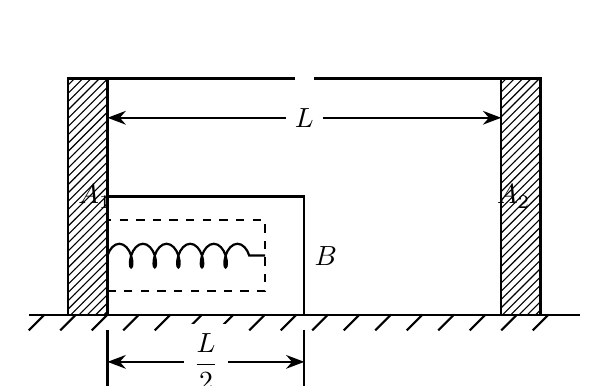
\begin{tikzpicture}[>=Stealth, thick]
    % 地面及阴影线
    \draw (-0.5, 0) -- (6.5, 0);
    \foreach \x in {-0.3, 0.1, ..., 6.3} {
        \draw (\x, 0) -- (\x-0.2, -0.2);
    }
    
    % 左侧壁 A1
    \draw[pattern=north east lines] (0, 0) rectangle (0.5, 3);
    \draw (0, 0) rectangle (0.5, 3);
    \node[right] at (0, 1.5) {$A_1$};
    
    % 右侧壁 A2
    \draw[pattern=north east lines] (5.5, 0) rectangle (6, 3);
    \draw (5.5, 0) rectangle (6, 3);
    \node[left] at (6, 1.5) {$A_2$};
    
    % 滑块 B
    \draw (0.5, 0) rectangle (3, 1.5);
    \node[right] at (3, 0.75) {$B$};
    
    % 滑块内部的弹簧与虚线框
    \draw[dashed] (0.5, 0.3) rectangle (2.5, 1.2);
    \draw[decorate, decoration={coil, aspect=0.5, segment length=3mm, amplitude=1.5mm}] (0.5, 0.75) -- (2.5, 0.75);
    
    % 顶部宽度标注 L
    \draw (0.5, 3) -- (5.5, 3) node[midway, fill=white] {};
    \draw[<->] (0.5, 2.5) -- (5.5, 2.5) node[midway, fill=white] {$L$};
    
    % 底部宽度标注 L/2
    \draw (0.5, -0.2) -- (0.5, -1);
    \draw (3, -0.2) -- (3, -1);
    \draw[<->] (0.5, -0.6) -- (3, -0.6) node[midway, fill=white] {$\dfrac{L}{2}$};
\end{tikzpicture}}\\[4pt]
{\small 图 3-51（题 3-18）}
\end{center}

\newpage

\pdfbookmark[1]{题 3-19}{prob3-19}
\textbf{3-19} 在水平冰面上兄弟俩作推车游戏, 哥哥质量 $m_{1}$ , 弟弟质量 $m_{2}$ , 小车质量 $m$ . 开始时哥哥与小车静止在同一地点, 弟弟静止在另一地点. 而后, 哥哥将小车朝着弟弟推去, 小车推出后相对于哥哥的速度大小为 $u$ . 弟弟接到小车后又将小车推向哥哥, 小车推出后相对于弟弟的速度大小仍为 $u$ . 哥哥接到小车后又再次将小车推向弟弟, 如此继续下去. 设冰面光滑, 且足够大.

(1) 若某次弟弟推出的小车恰好追不上哥哥, 试求三者各自的运动速度大小;

(2) 若无论 $u$ 取什么样的非零值, 弟弟第一次推出的小车都是恰好追不上哥哥，试给出 $m_{1}, m_{2}, m$ 之间需满足的关系式.

\newpage

\pdfbookmark[1]{题 3-20}{prob3-20}
\textbf{3-20} 质量 $m$ 的均匀圆环形光滑细管道放在光滑水平大桌面上，管内有两个质量同为 $m$ 的小球 $A$ 和 $B$ 位于一条直径的两端. 开始时管道静止， $A$ 和 $B$ 沿着切线方向有相同速度 $v_0$ ，如图 3-52 所示． $A, B$ 间碰撞的恢复系数 $e = \frac{\sqrt{3}}{3}$ ，试求：

(1) $A$, $B$ 第一次碰撞前瞬间的相对速度大小 $u$;

(2) $A$, $B$ 第二次碰撞前瞬间各自相对大桌面的速度大小 $v'$ .

\begin{center}
\resizebox{0.35\textwidth}{!}{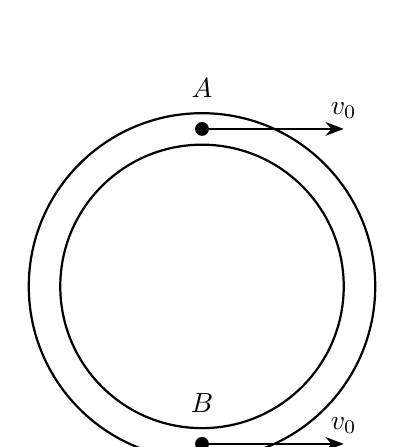
\begin{tikzpicture}[>=Stealth, thick]
    % 环形轨道
    \draw (0, 0) circle (2.2);
    \draw (0, 0) circle (1.8);
    
    % 质点 A 与速度
    \fill (0, 2.0) circle (2.5pt);
    \node[above=2pt] at (0, 2.2) {$A$};
    \draw[->] (0, 2.0) -- (1.8, 2.0) node[above] {$v_0$};
    
    % 质点 B 与速度
    \fill (0, -2.0) circle (2.5pt);
    \node[above=2pt] at (0, -1.8) {$B$};
    \draw[->] (0, -2.0) -- (1.8, -2.0) node[above] {$v_0$};
\end{tikzpicture}}\\[4pt]
{\small 图 3-52（题 3-20）}
\end{center}

\newpage

\pdfbookmark[1]{题 3-21}{prob3-21}
\textbf{3-21} 小球 $A, B$ 在光滑水平面上沿同一直线朝着对方运动， $A$ 球质量大于 $B$ 球质量。已知碰前两球动能相同，碰后 $A$ 球速度为零， $B$ 球速度不为零，试求 $A$ 球质量与 $B$ 球质量之比 $\gamma$ 。

\newpage

\pdfbookmark[1]{题 3-22}{prob3-22}
\textbf{3-22} 长平板在水平方向上以恒定的速度 $v_{0}$ 朝右运动，板上方 $H$ 高处有一小球自静止自由下落与平板碰撞。已知球与平板间摩擦因数 $\mu=0.1$ ，小球反弹高度仍为 $H$，试确定图 3-53 中小球反弹抛射角 $\phi$ 的正切 $\tan\phi$ 与 $\sqrt{H}$ 之间的函数关系。

\begin{center}
\resizebox{0.50\textwidth}{!}{\begin{tikzpicture}[>=Stealth, thick]
    % 地面及阴影
    \draw (-2.5, 0) -- (4, 0);
    \foreach \x in {-2.3, -1.9, ..., 3.7} {
        \draw (\x, 0) -- (\x-0.2, -0.2);
    }
    
    % 平板
    \draw (-1.5, 0) rectangle (2.5, 0.3);
    
    % 平板上固定的斜劈角 \phi
    \draw (0.2, 0.3) -- (1.8, 1.2);
    \draw (0.8, 0.3) arc (0:29:0.6);
    \node at (1.0, 0.55) {$\phi$};
    
    % 下落质点及竖直虚线
    \fill (0.2, 3) circle (2pt);
    \draw[dashed] (0.2, 3) -- (0.2, 0.3) node[midway, left] {$H$};
    
    % 平板速度 v_0
    \draw[->] (3.0, 0.6) -- (4.0, 0.6) node[above] {$v_0$};
\end{tikzpicture}}\\[4pt]
{\small 图 3-53（题 3-22）}
\end{center}

\newpage

\pdfbookmark[1]{题 3-23}{prob3-23}
\textbf{3-23} 一斜面体静放在光滑水平地面上, 斜面倾角 $\theta = 15^{\circ}$ . 如图 3-54 所示, 小球从静止自由下落到光滑斜面, 下落高度 $h = 1.60 \mathrm{~m}$ , 碰撞点距地面高度 $H = 1.00 \mathrm{~m}$ . 小球与斜面法向碰撞恢复系数 $e = 0.60$ , 碰后斜面体不离地, 小球与斜面体的质量比 $m / M = 0.5$ .

(1) 求碰后小球反弹速度和斜面体获得的速度；

(2) 求碰后小球最高位置相对原碰撞点的高度；

(3) 判断小球碰后将落于斜面还是落于地面?

\begin{center}
\resizebox{0.47\textwidth}{!}{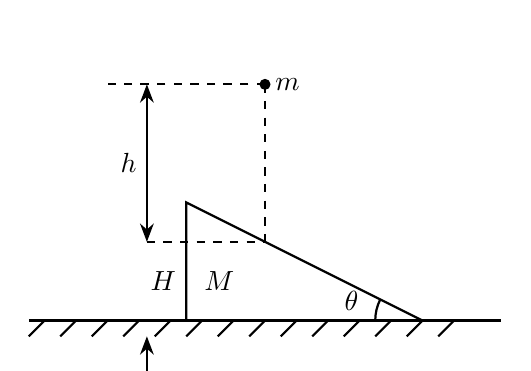
\begin{tikzpicture}[>=Stealth, thick]
    % 地面及阴影
    \draw (-1, 0) -- (5, 0);
    \foreach \x in {-0.8, -0.4, ..., 4.8} {
        \draw (\x, 0) -- (\x-0.2, -0.2);
    }
    
    % 斜面 M
    \draw (1, 0) -- (4, 0) -- (1, 1.5) -- cycle;
    \node[right] at (1.1, 0.5) {$M$};
    \node[left] at (1, 0.5) {$H$};
    
    % 角度 \theta
    \draw (3.4, 0) arc (180:153.4:0.6); % arctan(1.5/3) ≈ 26.6°, 180-26.6 = 153.4
    \node at (3.1, 0.25) {$\theta$};
    
    % 质点 m 及下落虚线
    \fill (2, 3) circle (2pt) node[right] {$m$};
    \draw[dashed] (2, 3) -- (2, 1);
    
    % 高度 h 标注辅助线
    \draw[dashed] (2, 3) -- (0, 3);
    \draw[dashed] (0.5, 1) -- (2, 1);
    \draw[<->] (0.5, 1) -- (0.5, 3) node[midway, left] {$h$};
    
    % 地面下方的短直立箭头
    \draw[->] (0.5, -0.8) -- (0.5, -0.2);
\end{tikzpicture}}\\[4pt]
{\small 图 3-54（题 3-23）}
\end{center}

\newpage

\pdfbookmark[1]{题 3-24}{prob3-24}
\textbf{3-24} 三个编号分别为 1,2,3 的相同匀质光滑小立方块，按图 3-55 所示方式放在光滑水平面上，直径与立方块边长相同的匀质光滑小圆柱块沿着图中对称方向以速度 $u_0$ 运动过来，接着便发生弹性碰撞。已知圆柱块质量是每一立方块质量的 2 倍，试求碰后各物块运动速度大小 $v_1, v_2, v_3$ 和 $u$ 。

\begin{center}
\resizebox{0.50\textwidth}{!}{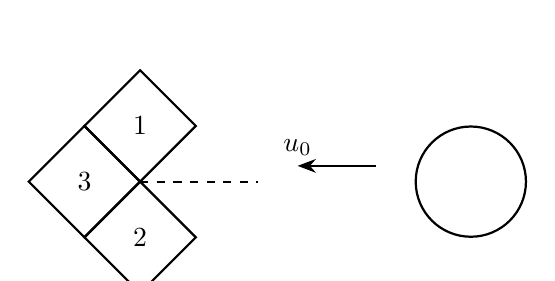
\begin{tikzpicture}[>=Stealth, thick]
    % 左侧三个拼接的正方形方块 (以45度角放置)
    % Block 3 (最左侧)
    \draw (-1.414, 0) -- (-0.707, 0.707) -- (0, 0) -- (-0.707, -0.707) -- cycle;
    \node at (-0.707, 0) {$3$};
    
    % Block 1 (右上)
    \draw (-0.707, 0.707) -- (0, 1.414) -- (0.707, 0.707) -- (0, 0) -- cycle;
    \node at (0, 0.707) {$1$};
    
    % Block 2 (右下)
    \draw (-0.707, -0.707) -- (0, 0) -- (0.707, -0.707) -- (0, -1.414) -- cycle;
    \node at (0, -0.707) {$2$};
    
    % 虚线轴心
    \draw[dashed] (0, 0) -- (1.5, 0);
    
    % 速度矢量 u_0
    \draw[->] (3.0, 0.2) -- (2.0, 0.2) node[above] {$u_0$};
    
    % 右侧圆环
    \draw (4.2, 0) circle (0.7);
\end{tikzpicture}}\\[4pt]
{\small 图 3-55（题 3-24）}
\end{center}

\newpage

\pdfbookmark[1]{题 3-25}{prob3-25}
\textbf{3-25} 在一水平面上有两根相互平行的固定导轨 $M_{1}N_{1}$ 和 $M_{2}N_{2}$ , 质量 $m_{1}$ 的物块 $P_{1}$ 穿在 $M_{1}N_{1}$ 上, 质量 $m_{2}$ 的物块 $P_{2}$ 穿在 $M_{2}N_{2}$ 上, $P_{1}$ 与 $P_{2}$ 间用一根不可伸长的轻绳连接, 开始时绳处于松弛状态. 今使 $P_{1}$ 获得沿导轨方向速度 $v_{0}, P_{2}$ 静止, 如图 3-56 所示. 设系统处处无摩擦, $P_{1}$ 运动一段时间后绳被拉直,其内产生拉力,同时使导轨与相应的物块间有力的作用,这些力的作用时间 $\Delta t$ 非常短.试就下述两种情况,计算 $\Delta t$ 刚结束时 $P_{1}$ 和 $P_{2}$ 运动速度 $u_{1}$ 和 $u_{2}$ .

(1) 绳的作用不损耗系统动能；

(2) 绳的作用使 $P_{1}$ 和 $P_{2}$ 沿绳长方向的速度相同.

\begin{center}
\resizebox{0.50\textwidth}{!}{\begin{tikzpicture}[>=Stealth, thick]
    % 上下平行轨道
    \draw (0, 2) node[left] {$M_1$} -- (5, 2) node[right] {$N_1$};
    \draw (0, 0) node[left] {$M_2$} -- (5, 0) node[right] {$N_2$};
    
    % 滑块 1 及其标签
    \draw (2.1, 1.85) rectangle (2.7, 2.15);
    \node[above] at (2.4, 2.15) {$P_1 \quad m_1$};
    
    % 滑块 2 及其标签
    \draw (2.1, -0.15) rectangle (2.7, 0.15);
    \node[below] at (2.4, -0.15) {$P_2 \quad m_2$};
    
    % 轻绳 (使用波浪线)
    \draw[decorate, decoration={snake, amplitude=1mm, segment length=4mm}] (2.4, 0.15) -- (2.4, 1.85);
    \node[left] at (2.3, 1) {轻绳};
    
    % 速度 v0 箭头
    \draw[->] (3.2, 1.5) -- (4.2, 1.5) node[midway, below] {$v_0$};
\end{tikzpicture}}\\[4pt]
{\small 图 3-56（题 3-25）}
\end{center}

\newpage

\pdfbookmark[1]{题 3-26}{prob3-26}
\textbf{3-26} 一架质量 $M = 810\mathrm{kg}$ 的直升飞机，靠螺旋桨的转动使 $S = 30\mathrm{m}^2$ 面积内的空气以 $v_{0}$ 速度向下运动，从而使飞机悬停在空中. 已知空气密度 $\rho_0 = 1.20\mathrm{kg / m^3}$ ，求 $v_{0}$ 大小，并计算发动机的最小功率 $p$ .

\newpage

\pdfbookmark[1]{题 3-27}{prob3-27}
\textbf{3-27} 内外半径几乎同为 $R$ 的竖直固定圆环管，底部有一质量为 $m$ 的小球，环内有根轻绳连接小球，绳的另一端从管的上方缺口水平引出，绳与管壁间摩擦可略。用力 $F$ 将绳拉出，并保证小球在运动的过程中始终具有原始的速率 $v_{0}$ 。设圆环管的外壁、内壁与小球的摩擦因数分别为 $\mu_{1}, \mu_{2}$ ，试求小球从图 3-57 所示位置到达最高位置的过程中，力 $F$ 所作功 $W$ 。

\begin{center}
\resizebox{0.42\textwidth}{!}{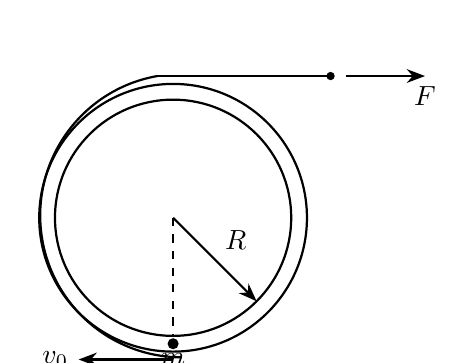
\begin{tikzpicture}[>=Stealth, thick]
    % 内外双层圆环
    \draw (0, 0) circle (1.5);
    \draw (0, 0) circle (1.7);
    
    % 半径 R 及中心辅助线
    \draw[dashed] (0, 0) -- (0, -1.5);
    \draw[->] (0, 0) -- (1.06, -1.06) node[midway, above right] {$R$};
    
    % 底部质点 m 及速度 v0
    \fill (0, -1.6) circle (2pt) node[below] {$m$};
    \draw[->] (0, -1.8) -- (-1.2, -1.8) node[left] {$v_0$};
    
    % 绕绳及水平拉力 F
    \draw (-0.2, 1.8) arc (100:270:1.8);
    \draw (-0.2, 1.8) -- (2, 1.8);
    \fill (2, 1.8) circle (1.5pt);
    \draw[->] (2.2, 1.8) -- (3.2, 1.8) node[below] {$F$};
\end{tikzpicture}}\\[4pt]
{\small 图 3-57（题 3-27）}
\end{center}

\newpage

\pdfbookmark[1]{题 3-28}{prob3-28}
\textbf{3-28} 在航天飞船上,如图 3-58 所示,有一个长 $l=20\ cm$ 的圆筒绕着与筒的长度方向垂直的轴 MN 以恒定的角速度$\omega = \frac{10}{3}\pi \mathrm{s}^{-1}$ 旋转. 筒的近轴端与轴相距 $d = 10\mathrm{cm}$ , 筒内装满非常黏稠、密度 $\rho = 1.2\mathrm{g/cm^3}$ 的液体. 有一个质量 $m' = 1.0\mathrm{mg}$ 、密度 $\rho' = 1.5\mathrm{g/cm^3}$ 的颗粒 $P$ , 从圆筒中央位置静止释放, 试求 $P$ 在到达筒端过程中克服液体黏性阻力所作功. 又问, 如果 $P$ 的密度 $\rho'' = 1.0\mathrm{g/cm^3}$ , 其他条件不变, 则 $P$ 在到达筒端过程中克服液体黏性阻力所作功又是多少?

\begin{center}
\resizebox{0.50\textwidth}{!}{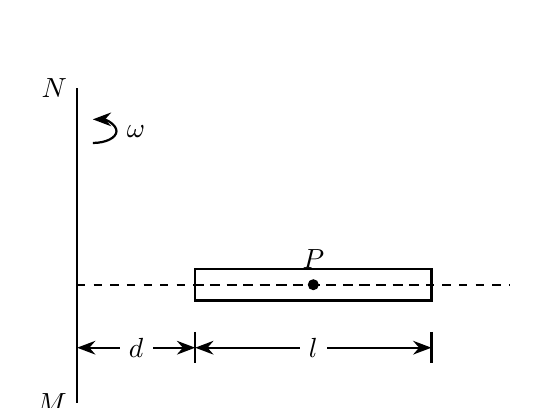
\begin{tikzpicture}[>=Stealth, thick]
    % 垂直旋转轴 MN
    \draw (0, -1.5) node[left] {$M$} -- (0, 2.5) node[left] {$N$};
    
    % 旋转角速度 \omega
    \draw[->] (0.2, 1.8) arc (-90:90:0.3 and 0.15);
    \node[right] at (0.5, 1.95) {$\omega$};
    
    % 中心水平虚线
    \draw[dashed] (0, 0) -- (5.5, 0);
    
    % 金属杆 P
    \draw (1.5, -0.2) rectangle (4.5, 0.2);
    \draw[dashed] (1.5, 0) -- (4.5, 0);
    \fill (3, 0) circle (2pt) node[above=2pt] {$P$};
    
    % 下方距离 d 与 l 的标注
    \draw[<->] (0, -0.8) -- (1.5, -0.8) node[midway, fill=white] {$d$};
    \draw[<->] (1.5, -0.8) -- (4.5, -0.8) node[midway, fill=white] {$l$};
    
    % 距离辅助短线
    \draw (0, -0.6) -- (0, -1);
    \draw (1.5, -0.6) -- (1.5, -1);
    \draw (4.5, -0.6) -- (4.5, -1);
\end{tikzpicture}}\\[4pt]
{\small 图 3-58（题 3-28）}
\end{center}

\newpage

\pdfbookmark[1]{题 3-29}{prob3-29}
\textbf{3-29} 两个核子之间的相互作用势能可表述为 $U(r) = -\frac{r_0}{r} U_0 \mathrm{e}^{-r / r_0}$ , 这便是汤川(Yukawa)势. 式中 $r_0 (r_0 = 1.5 \times 10^{-15} \mathrm{~m})$ , $U_0 (U_0 = 50 \mathrm{MeV})$ 均为常量.

(1) 给出两个核子之间相互作用力的表达式；

(2) 计算当 $r=2r_{0},5r_{0},10r_{0}$ 时的作用力与 $r=r_{0}$ 时的作用力之比, 由此可见此种力的短程特征.

\newpage

\pdfbookmark[1]{题 3-30}{prob3-30}
\textbf{3-30} 地面上有一固定的点电荷 $A$. $A$ 的正上方有另一带电质点 $B$，在重力和库仑斥力作用下，$B$ 在 $A$ 的正上方 $H$ 到 H/2 高度间往返运动，试求 $B$ 的最大运动速度 $v_{max}$ .

\newpage

\pdfbookmark[1]{题 3-31}{prob3-31}
\textbf{3-31} 将劲度系数为 $k$ 、自由长度为 $L$ 、质量为 $m$ 的均匀柱形弹性体竖直朝下，上端固定，下端自由. 开始时弹性体处处无形变，而后在重力作用下各部位发生运动和形变,因为空气阻力等作用,最后弹性体处于静止状态,试求弹性体的弹性势能和重力势能的各自增量.

\newpage

\pdfbookmark[1]{题 3-32}{prob3-32}
\textbf{3-32} 各边长为 $l$ 的匀质立方体大木块, 如图 3-59 所示, 对半切成两块, 将上表面为 $AB_{1}CB_{2}$ 斜平面的一块留下放在水平面上, 其质量为 $2m$ . 沿 $AB_{1}, AB_{2}, B_{1}C, B_{2}C$ 设置四根斜直细管道, 质量均为 $m$ 的两个小球同时从 $A$ 端静止释放, 分别沿 $AB_{1}C, AB_{2}C$ 管道滑下, 它们在 $B_{1}, B_{2}$ 处可光滑迅速地拐弯.

(1) 设木块固定在水平面上，管道平直部分与各小球之间的摩擦因数同为 $\mu$ ，试问 $\mu$ 为何值，小球才能滑下？并计算小球到达 $C$ 处时的速度.

(2) 设木块与水平面光滑接触, 管道内处处无摩擦, 试求小球到达 $C$ 处时相对地面的速度大小.

\begin{center}
\resizebox{0.40\textwidth}{!}{\begin{tikzpicture}[>=Stealth, thick, line join=round]
    % 底部支撑面
    \draw (-1.5, -0.8) -- (2.5, -0.8) -- (3.5, 0.6) -- (-0.5, 0.6) -- cycle;
    
    % 立方体可见边
    \draw (0, 0) node[left] {$C$} -- (2, 0) node[right] {$B_1$} -- (2.8, 0.8) -- (2.8, 2.8) node[right] {$A$} -- (0.8, 2.8) node[left] {$B_2$} -- (0, 2) -- cycle;
    \draw (2, 0) -- (2, 2) -- (2.8, 2.8);
    \draw (0, 2) -- (2, 2);
    
    % 立方体不可见边 (背面虚线)
    \draw[dashed] (0, 0) -- (0.8, 0.8) -- (2.8, 0.8);
    \draw[dashed] (0.8, 0.8) -- (0.8, 2.8);
    
    % 内部与表面对角线
    \draw (0, 0) -- (2.8, 2.8);
    \draw (0, 0) -- (2, 0) -- (2.8, 2.8) -- cycle;
    \draw[dashed] (0, 0) -- (0.8, 2.8) -- (2.8, 2.8);
    
    % 边长 l 标注
    \node[left] at (0, 1) {$l$};
    \node[above left] at (0.4, 2.4) {$l$};
    \node[above] at (1.8, 2.8) {$l$};
\end{tikzpicture}}\\[4pt]
{\small 图 3-59（题 3-32）}
\end{center}

\newpage

\pdfbookmark[1]{题 3-33}{prob3-33}
\textbf{3-33} 如图 3-60 所示, 质量 $2m$ 的小环套在水平光滑的固定细杆上, 并用长 $l$ 的轻线与质量为 $m$ 的小球相连. 今将轻线沿水平拉直, 使小球从与环等高处由静止释放, 试问当轻线与水平杆夹角为 $\theta$ 时线中张力 $T$ 为多大?

\begin{center}
\resizebox{0.36\textwidth}{!}{\begin{tikzpicture}[>=Stealth, thick]
    % 水平直杆
    \draw (0, 0) -- (4.5, 0);
    
    % 圆环 2m
    \draw (1.5, 0) ellipse (0.15 and 0.25);
    \node[above] at (1.5, 0.25) {$2m$};
    
    % 细线与悬挂的质点 m
    \draw (1.5, -0.25) -- (3.5, -0.25);
    \fill (3.5, -0.25) circle (2pt) node[below right] {$m$};
    
    % 细线长度 l 标注
    \node[below] at (2.5, -0.25) {$l$};
\end{tikzpicture}}\\[4pt]
{\small 图 3-60（题 3-33）}
\end{center}

\newpage

\pdfbookmark[1]{题 3-34}{prob3-34}
\textbf{3-34} 在一个带有活塞的固定柱形汽缸内有一单原子分子沿着汽缸的长度方向往返运动,它与汽缸左壁及活塞均作弹性正碰撞.

(1) 如图 3-61 所示, 设汽缸的初始长度为 $l_{0}$ , 活塞推进速度为常量 $u$ , 分子从活塞近旁以 $v_{0} \gg u$ 的初始速率朝汽缸左壁运动. 略去重力影响, 试确定分子与活塞多次碰撞后, 其速率 $v$ 与汽缸长度 $l$ 之间的关系.

(2) 设汽缸截面积为 $S$，则汽缸初始体积 $V_{0}=S \cdot l_{0}$ ，汽缸长度为 $l$ 时的体积 $V=S \cdot l$ 。再为该分子引入“温度”量 $T$，使其正比于分子的动能，试求 $T$ 与 $V$ 之间的关系。

\begin{center}
\resizebox{0.42\textwidth}{!}{\begin{tikzpicture}[>=Stealth, thick]
    % 气缸外壁 (左侧封闭，右侧开口)
    \draw (0, 0) -- (4, 0);
    \draw (0, 2) -- (4, 2);
    \draw (0, 0) -- (0, 2);
    
    % 活塞主体 (填充剖面线)
    \fill[pattern=north east lines] (2.5, 0) rectangle (3, 2);
    \draw (2.5, 0) rectangle (3, 2);
    
    % 活塞外部连杆
    \fill[pattern=north east lines] (3, 0.8) rectangle (4.2, 1.2);
    \draw (3, 0.8) -- (4.2, 0.8);
    \draw (3, 1.2) -- (4.2, 1.2);
    \draw (4.2, 0.8) -- (4.2, 1.2);
    
    % 活塞向左运动速度 u
    \draw[->] (5.2, 1) -- (4.4, 1) node[midway, above] {$u$};
    
    % 气缸内部质点及向左速度 v0
    \fill (2.2, 1) circle (2pt);
    \draw[->] (2.0, 1) -- (1.2, 1) node[midway, above] {$v_0$};
    
    % 初始长度 l0 标注
    \draw[<->] (0, 2.3) -- (2.5, 2.3) node[midway, fill=white] {$l_0$};
    
    % l0 的上下辅助线
    \draw (0, 2) -- (0, 2.6);
    \draw (2.5, 2) -- (2.5, 2.6);
\end{tikzpicture}}\\[4pt]
{\small 图 3-61（题 3-34）}
\end{center}

\newpage

\pdfbookmark[1]{题 3-35}{prob3-35}
\textbf{3-35} 光滑水平桌面上静止放置若干个相同的匀质光滑小球，打击其中某个球，与别的球逐个弹性碰撞经一闭合路线后又可停在原位置上，试问至少需放多少个球？给出一种球的放置图.

\newpage

\pdfbookmark[1]{题 3-36}{prob3-36}
\textbf{3-36} 小球从水平地面上以初速 $v_{0}$ 斜抛出去, 小球落地时在竖直方向上发生的非弹性碰撞恢复系数为 $e$, 小球与地面间的摩擦因数为 $\mu$ . 若要求小球第一次与地面碰撞后能竖直弹起, 试求小球可能达到的最大水平射程 $s_{max}$ .

\newpage

\pdfbookmark[1]{题 3-37}{prob3-37}
\textbf{3-37} 如图 3-62 所示, 质量 $M$、倾角 $\phi$ 的斜面体静放在光滑水平面上, 质量 $m$ 的小球以水平速度 $v_{0}$ 与斜面发生碰撞, 设小球与斜面间无摩擦, 且碰撞无动能损失.

(1) 试求碰后小球沿斜面方向的速度 $v_{\parallel}$ 和垂直于斜面方向速度 $v_{\perp}$ ，以及斜面体沿地面运动速度 $u$；

(2) $M, m, \phi$ 之间满足什么样的关系，能使小球碰后速度竖直向上？

\begin{center}
\resizebox{0.50\textwidth}{!}{\begin{tikzpicture}[>=Stealth, thick]
    % 地面及阴影
    \draw (-2.5, 0) -- (4.5, 0);
    \foreach \x in {-2.3, -1.9, ..., 4.3} {
        \draw (\x, 0) -- (\x-0.2, -0.2);
    }
    
    % 斜面 M
    \draw (0, 0) -- (4, 0) -- (4, 2) -- cycle;
    \node at (3.5, 0.6) {$M$};
    
    % 角度 \phi
    \draw (0.6, 0) arc (0:26.5:0.6); % arctan(2/4) ≈ 26.5°
    \node at (0.9, 0.25) {$\phi$};
    
    % 质点 m
    \fill (-1.5, 1) circle (2pt);
    \node[above] at (-1.5, 1.1) {$m$};
    
    % 速度 v0 箭头
    \draw[->] (-1.3, 1) -- (-0.1, 1) node[midway, above] {$v_0$};
\end{tikzpicture}}\\[4pt]
{\small 图 3-62（题 3-37）}
\end{center}

\newpage

\pdfbookmark[1]{题 3-38}{prob3-38}
\textbf{3-38} 质量相同的两个小球 $A$ 和 $B$ 用长 $L$ 轻绳连接, 开始时都静止在光滑的水平桌面边缘. 今使 $B$ 球以 $v_{0} = \sqrt{\frac{gL}{2\sqrt{2}}}$ 的初速水平抛出, 如图 3-63 所示. 设绳不损耗机械能, 试求绳伸直后很短时间内因绳的作用而使 $A, B$ 各自具有的速度 $\pmb{v}_{A}, \pmb{v}_{B}$ .

\begin{center}
\resizebox{0.42\textwidth}{!}{\begin{tikzpicture}[>=Stealth, thick]
    % 平台及边缘
    \draw (-2.5, 0) -- (1.5, 0) -- (1.5, -2.5);
    
    % 质点 A
    \fill (0, 0.15) circle (0.15);
    \node[above] at (0, 0.3) {$A$};
    
    % 质点 B
    \fill (1.2, 0.15) circle (0.15);
    \node[above] at (1.2, 0.3) {$B$};
    
    % 弹簧 (连接 A 和 B)
    \draw[decorate, decoration={coil, aspect=0.5, segment length=3mm, amplitude=1.2mm}] (0.15, 0.15) -- (1.05, 0.15);
    
    % 速度 v0 箭头
    \draw[->] (1.8, 0.15) -- (2.8, 0.15) node[midway, below] {$v_0$};
\end{tikzpicture}}\\[4pt]
{\small 图 3-63（题 3-38）}
\end{center}


\end{document}
